\documentclass[12pt, twoside, openright]{report} %fuente a 12pt, formato doble pagina y chapter a la derecha
\raggedbottom % No ajustar el contenido con un salto de pagina

% MÁRGENES: 2,5 cm sup. e inf.; 3 cm izdo. y dcho.
\usepackage[
a4paper,
vmargin=2.5cm,
hmargin=3cm
]{geometry}

% INTERLINEADO: Estrecho (6 ptos./interlineado 1,15) o Moderado (6 ptos./interlineado 1,5)
\renewcommand{\baselinestretch}{1.15}
\parskip=6pt

% DEFINICIÓN DE COLORES para portada y listados de código
\usepackage[table]{xcolor}
\definecolor{azulUC3M}{RGB}{0,0,102}
\definecolor{gray97}{gray}{.97}
\definecolor{gray75}{gray}{.75}
\definecolor{gray45}{gray}{.45}

% Soporte para GENERAR PDF/A
\usepackage[a-1b]{pdfx}

% ENLACES
\usepackage{hyperref}
\hypersetup{colorlinks=true,
	linkcolor=black, % enlaces a partes del documento (p.e. índice) en color negro
	urlcolor=blue} % enlaces a recursos fuera del documento en azul

% Añadir pdfs como partes del documento
\usepackage{pdfpages}

% Quitar la indentación de principio de los parrafos
\setlength{\parindent}{0em}

% EXPRESIONES MATEMATICAS
\usepackage{amsmath,amssymb,amsfonts,amsthm}

\usepackage{txfonts} 
\usepackage[T1]{fontenc}
\usepackage[utf8]{inputenc}

% Insertar graficas y fotos
\usepackage{tikz}
\usepackage{pgfplots}

\usepackage[spanish, es-tabla]{babel} 
\usepackage[babel, spanish=spanish]{csquotes}
\AtBeginEnvironment{quote}{\small}

% diseño de PIE DE PÁGINA
\usepackage{fancyhdr}
\pagestyle{fancy}
\fancyhf{}
\renewcommand{\headrulewidth}{0pt}
\fancyfoot[LO,RE]{\thepage}
\fancypagestyle{plain}{\pagestyle{fancy}}

% DISEÑO DE LOS TÍTULOS de las partes del trabajo (capítulos y epígrafes o subcapítulos)
\usepackage{titlesec}
\usepackage{titletoc}
\titleformat{\chapter}[block]
{\large\bfseries\filcenter}
{\thechapter.}
{5pt}
{\MakeUppercase}
{}
\titlespacing{\chapter}{0pt}{0pt}{*3}
\titlecontents{chapter}
[0pt]                                               
{}
{\contentsmargin{0pt}\thecontentslabel.\enspace\uppercase}
{\contentsmargin{0pt}\uppercase}                        
{\titlerule*[.7pc]{.}\contentspage}                 

\titleformat{\section}
{\bfseries}
{\thesection.}
{5pt}
{}
\titlecontents{section}
[5pt]                                               
{}
{\contentsmargin{0pt}\thecontentslabel.\enspace}
{\contentsmargin{0pt}}
{\titlerule*[.7pc]{.}\contentspage}

\titleformat{\subsection}
{\normalsize\bfseries}
{\thesubsection.}
{5pt}
{}
\titlecontents{subsection}
[10pt]                                               
{}
{\contentsmargin{0pt}                          
	\thecontentslabel.\enspace}
{\contentsmargin{0pt}}                        
{\titlerule*[.7pc]{.}\contentspage}  


% DISEÑO DE TABLAS.
\usepackage{multirow} % permite combinar celdas 
\usepackage{caption} % para personalizar el título de tablas y figuras
\usepackage{floatrow} % utilizamos este paquete y sus macros \ttabbox y \ffigbox para alinear los nombres de tablas y figuras de acuerdo con el estilo definido. Para su uso ver archivo de ejemplo 
\usepackage{array} % con este paquete podemos definir en la siguiente línea un nuevo tipo de columna para tablas: ancho personalizado y contenido centrado
\newcolumntype{P}[1]{>{\centering\arraybackslash}p{#1}}
\DeclareCaptionFormat{upper}{#1#2\uppercase{#3}\par}

% Diseño de tabla para ingeniería
\captionsetup[table]{
	format=hang,
	name=Tabla,
	justification=centering,
	labelsep=colon,
	width=.75\linewidth,
	labelfont=small,
	font=small,
}

% DISEÑO DE FIGURAS.
\usepackage{graphicx}
\graphicspath{{img/}} %ruta a la carpeta de imágenes

% Diseño de figuras para ingeniería
\captionsetup[figure]{
	format=hang,
	name=Fig.,
	singlelinecheck=off,
	labelsep=colon,
	labelfont=small,
	font=small		
}

% NOTAS A PIE DE PÁGINA
\usepackage{chngcntr} %para numeración continua de las notas al pie
\counterwithout{footnote}{chapter}

% LISTADOS DE CÓDIGO
% soporte y estilo para listados de código. Más información en https://es.wikibooks.org/wiki/Manual_de_LaTeX/Listados_de_código/Listados_con_listings
\usepackage{listings}

% definimos un estilo de listings
\lstdefinestyle{estilo}{ frame=Ltb,
	framerule=0pt,
	aboveskip=0.5cm,
	framextopmargin=3pt,
	framexbottommargin=3pt,
	framexleftmargin=0.4cm,
	framesep=0pt,
	rulesep=.4pt,
	backgroundcolor=\color{gray97},
	rulesepcolor=\color{black},
	%
	basicstyle=\ttfamily\footnotesize,
	keywordstyle=\bfseries,
	stringstyle=\ttfamily,
	showstringspaces = false,
	commentstyle=\color{gray45},     
	%
	numbers=left,
	numbersep=15pt,
	numberstyle=\tiny,
	numberfirstline = false,
	breaklines=true,
	xleftmargin=\parindent
}

\captionsetup[lstlisting]{font=small, labelsep=period}
% fijamos el estilo a utilizar 
\lstset{style=estilo}
\renewcommand{\lstlistingname}{\uppercase{Código}}

\pgfplotsset{compat=1.17} 
%-------------
%	DOCUMENTO
%-------------

\begin{document}
\pagenumbering{roman} % Se utilizan cifras romanas en la numeración de las páginas previas al cuerpo del trabajo
	
%----------
%	PORTADA
%----------	
\begin{titlepage}
	\begin{sffamily}
	\color{azulUC3M}
	\begin{center}
		\begin{figure}[H] %incluimos el logotipo de la Universidad
			\makebox[\textwidth][c]{
\includegraphics[width=16cm]{Portada_Logo.png}}
		\end{figure}
		\vspace{2.5cm}
		\begin{Large}
			Grado en Ingeniería Informática\\			
			2020-2021\\
			\vspace{2cm}		
			\textsl{Apuntes}\\
			\bigskip
		\end{Large}
		 	{\Huge Sistemas Operativos}\\
		 	\vspace*{0.5cm}
	 		\rule{10.5cm}{0.1mm}\\
			\vspace*{0.9cm}
			{\LARGE Jorge Rodríguez Fraile\footnote{\href{mailto:100405951@alumnos.uc3m.es}{Universidad: 100405951@alumnos.uc3m.es}  |  \href{mailto:jrf1616@gmail.com}{Personal: jrf1616@gmail.com}}}\\ 
			\vspace*{1cm}
	\end{center}
	\vfill
	\color{black}
		
\includegraphics[width=4.2cm]{img/creativecommons.png}\\
		Esta obra se encuentra sujeta a la licencia Creative Commons\\ \textbf{Reconocimiento - No Comercial - Sin Obra Derivada}
	\end{sffamily}
\end{titlepage}

%----------
%	ÍNDICES
%----------	

%--
% Índice general
%-
\tableofcontents
\thispagestyle{fancy}

%----------
%	TRABAJO
%----------	
\pagenumbering{arabic} % numeración con múmeros arábigos para el resto de la publicación	


%----------
%	COMENZAR A ESCRIBIR AQUI
%----------	


\part{Información}
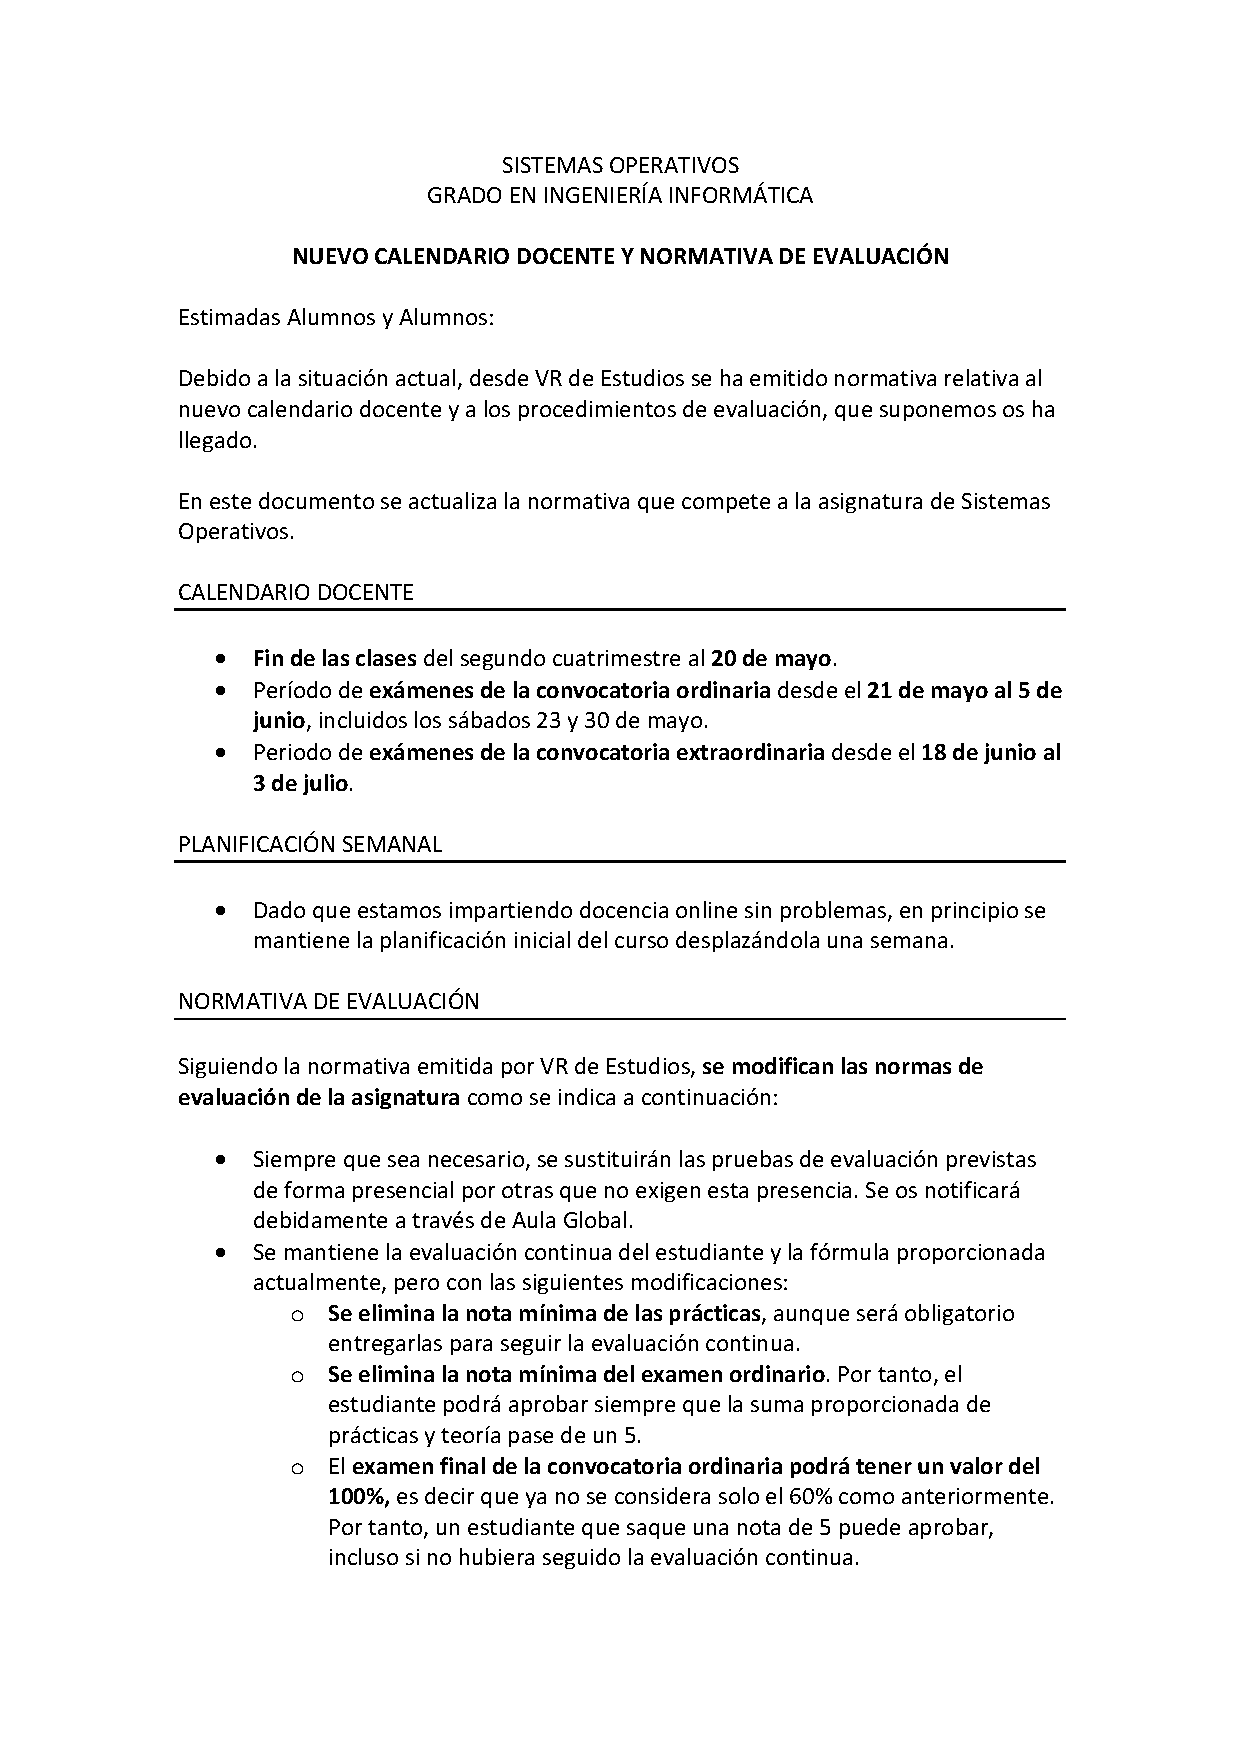
\includepdf[pages=-]{docs/Normativa-nueva.pdf}
\includepdf[pages=-]{docs/Sistemas_Operativos-2019-cronogramas.pdf}

\includepdf[pages=-]{docs/presentacion-ssoo.pdf}

\part{Resúmenes}
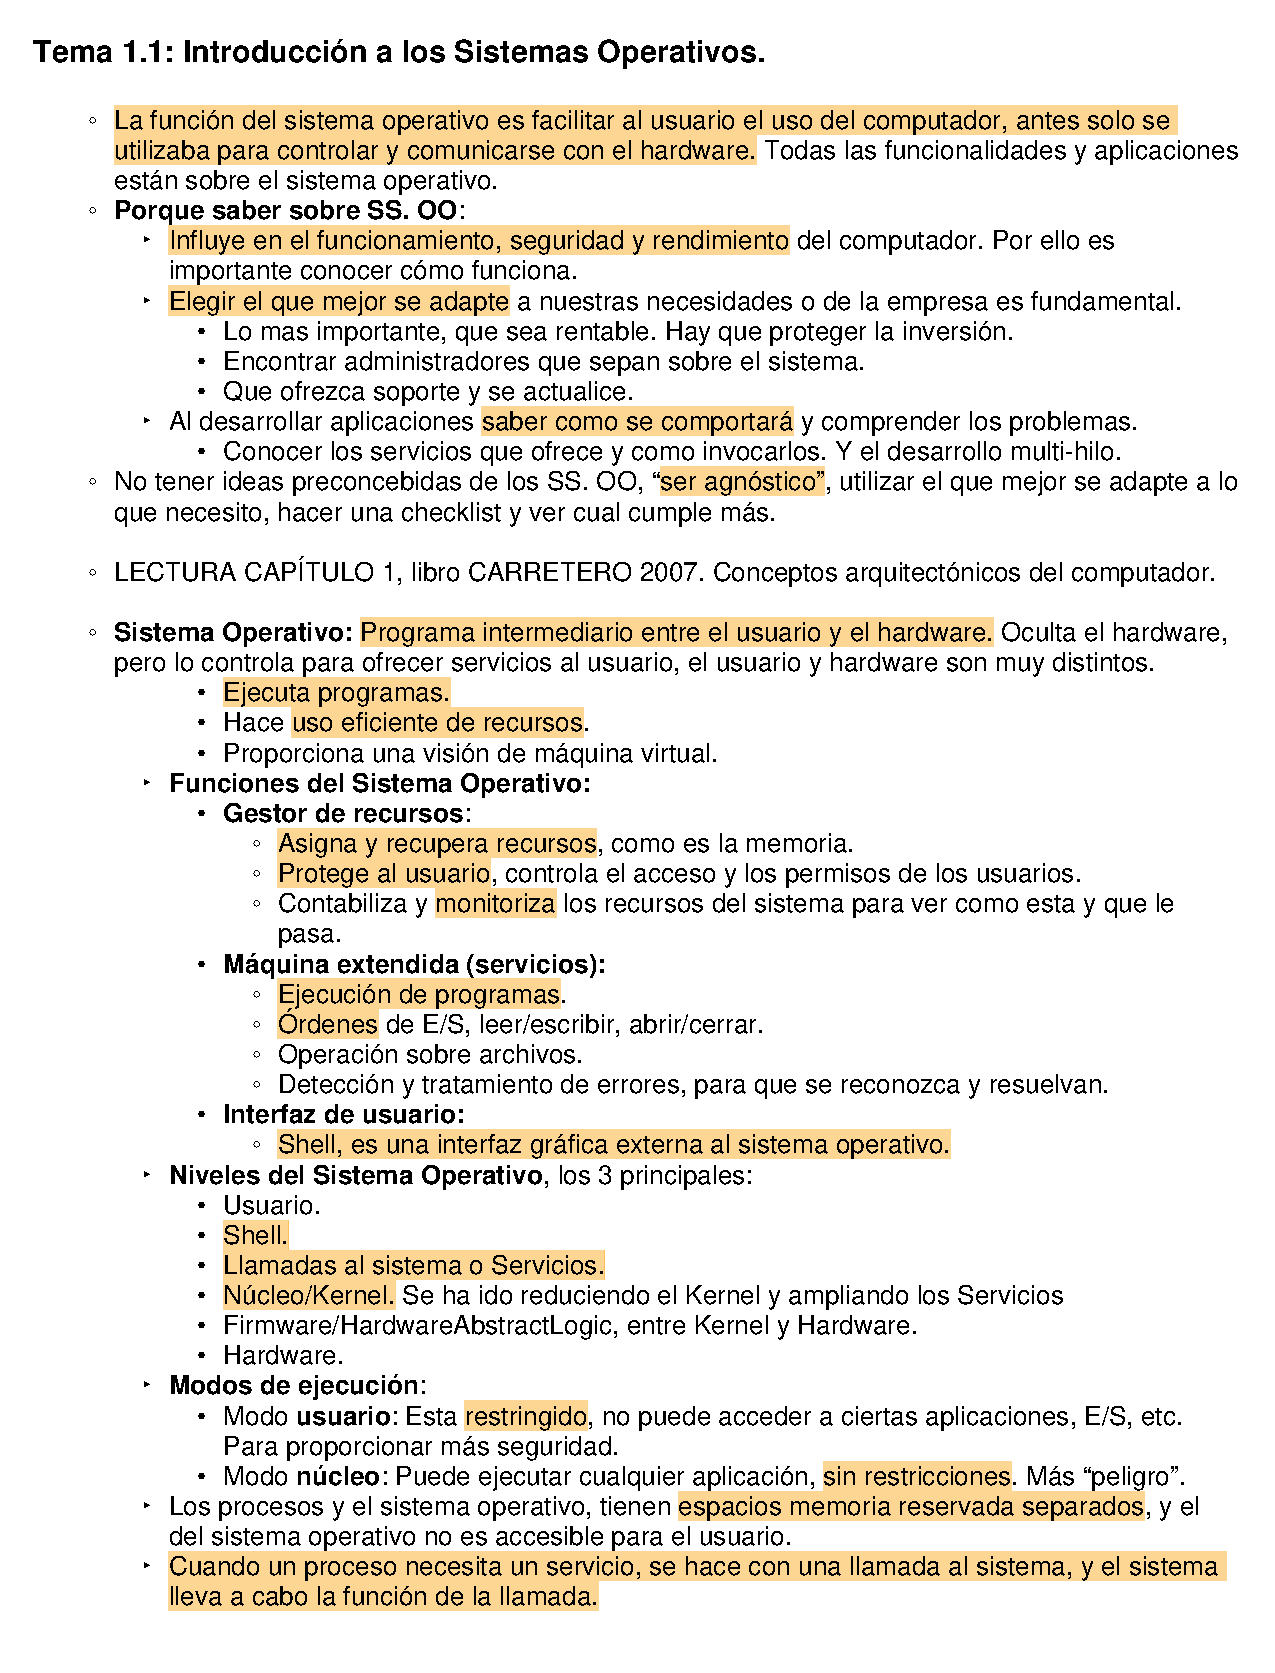
\includepdf[pages=-]{docs/Tema_1_SO.pdf}
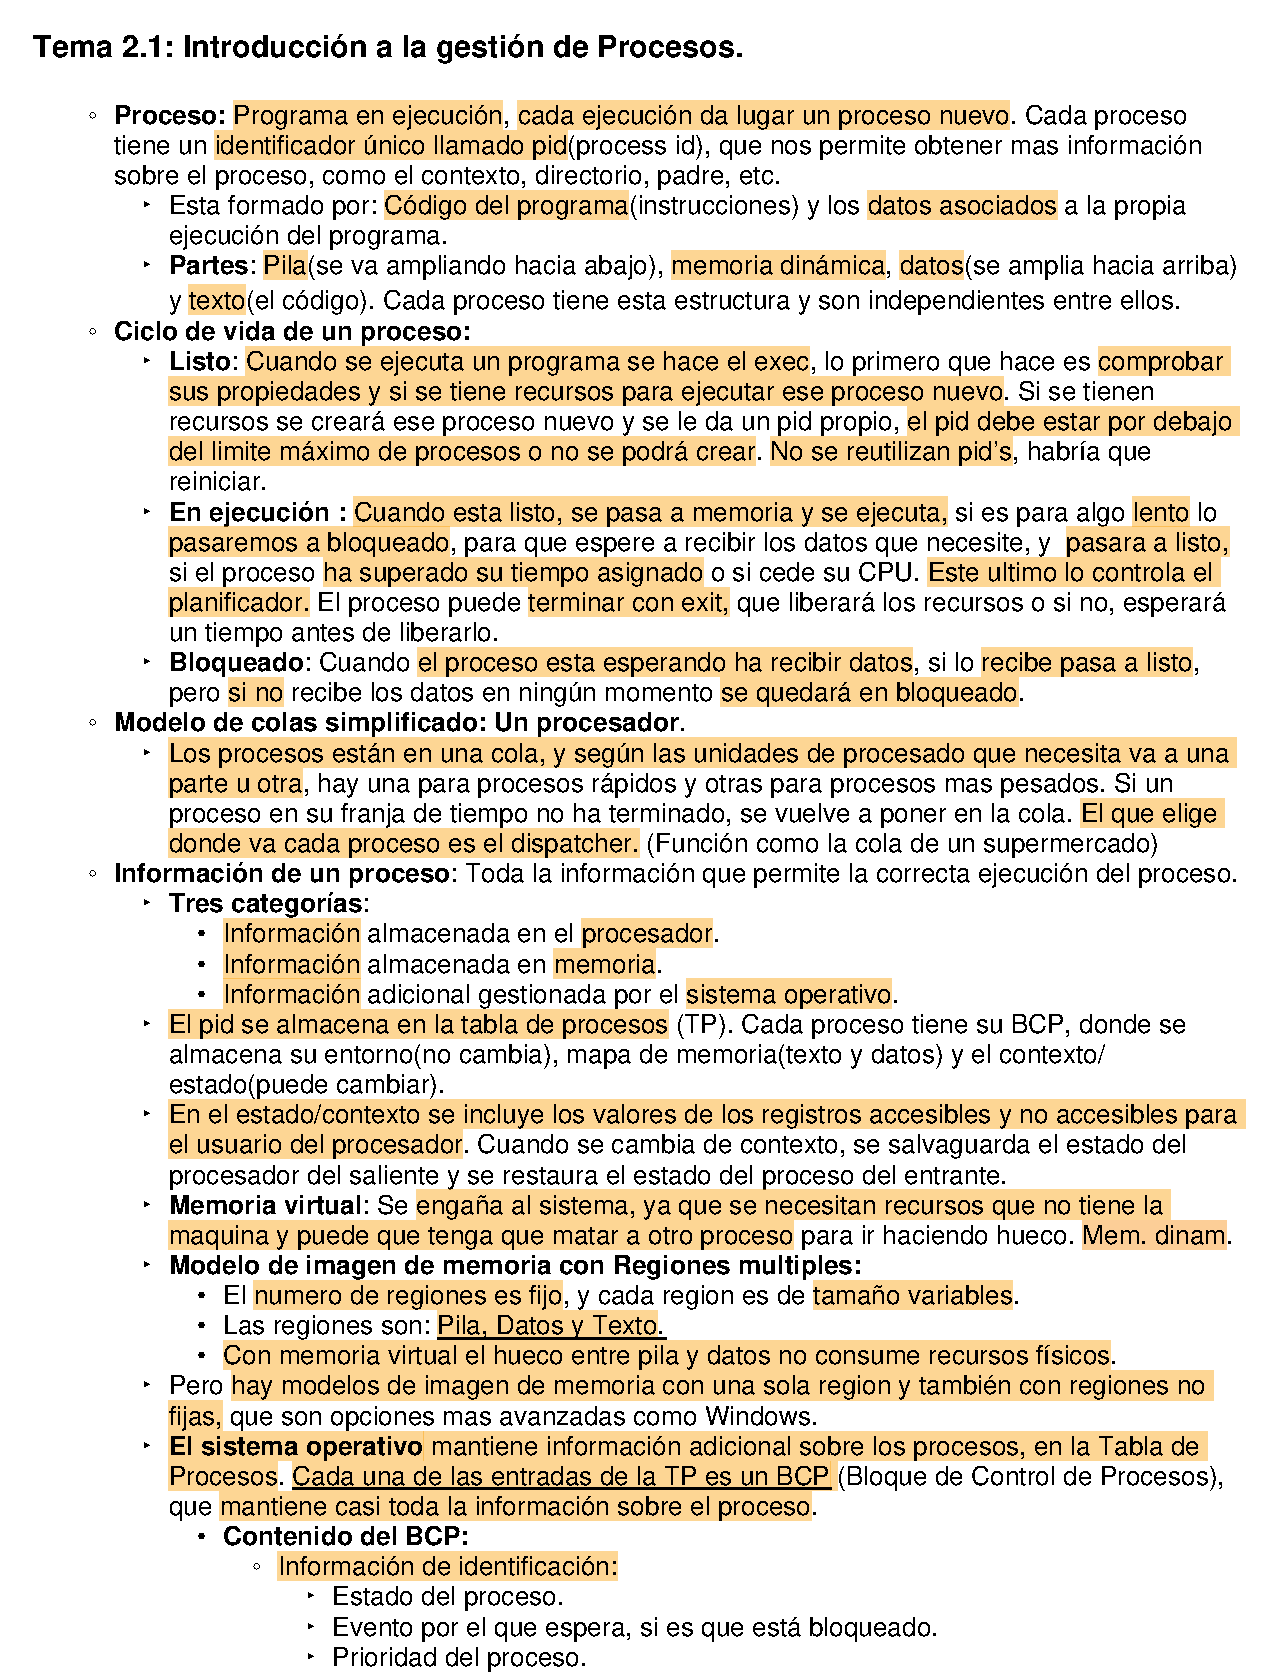
\includepdf[pages=-]{docs/Tema_2_SO.pdf}
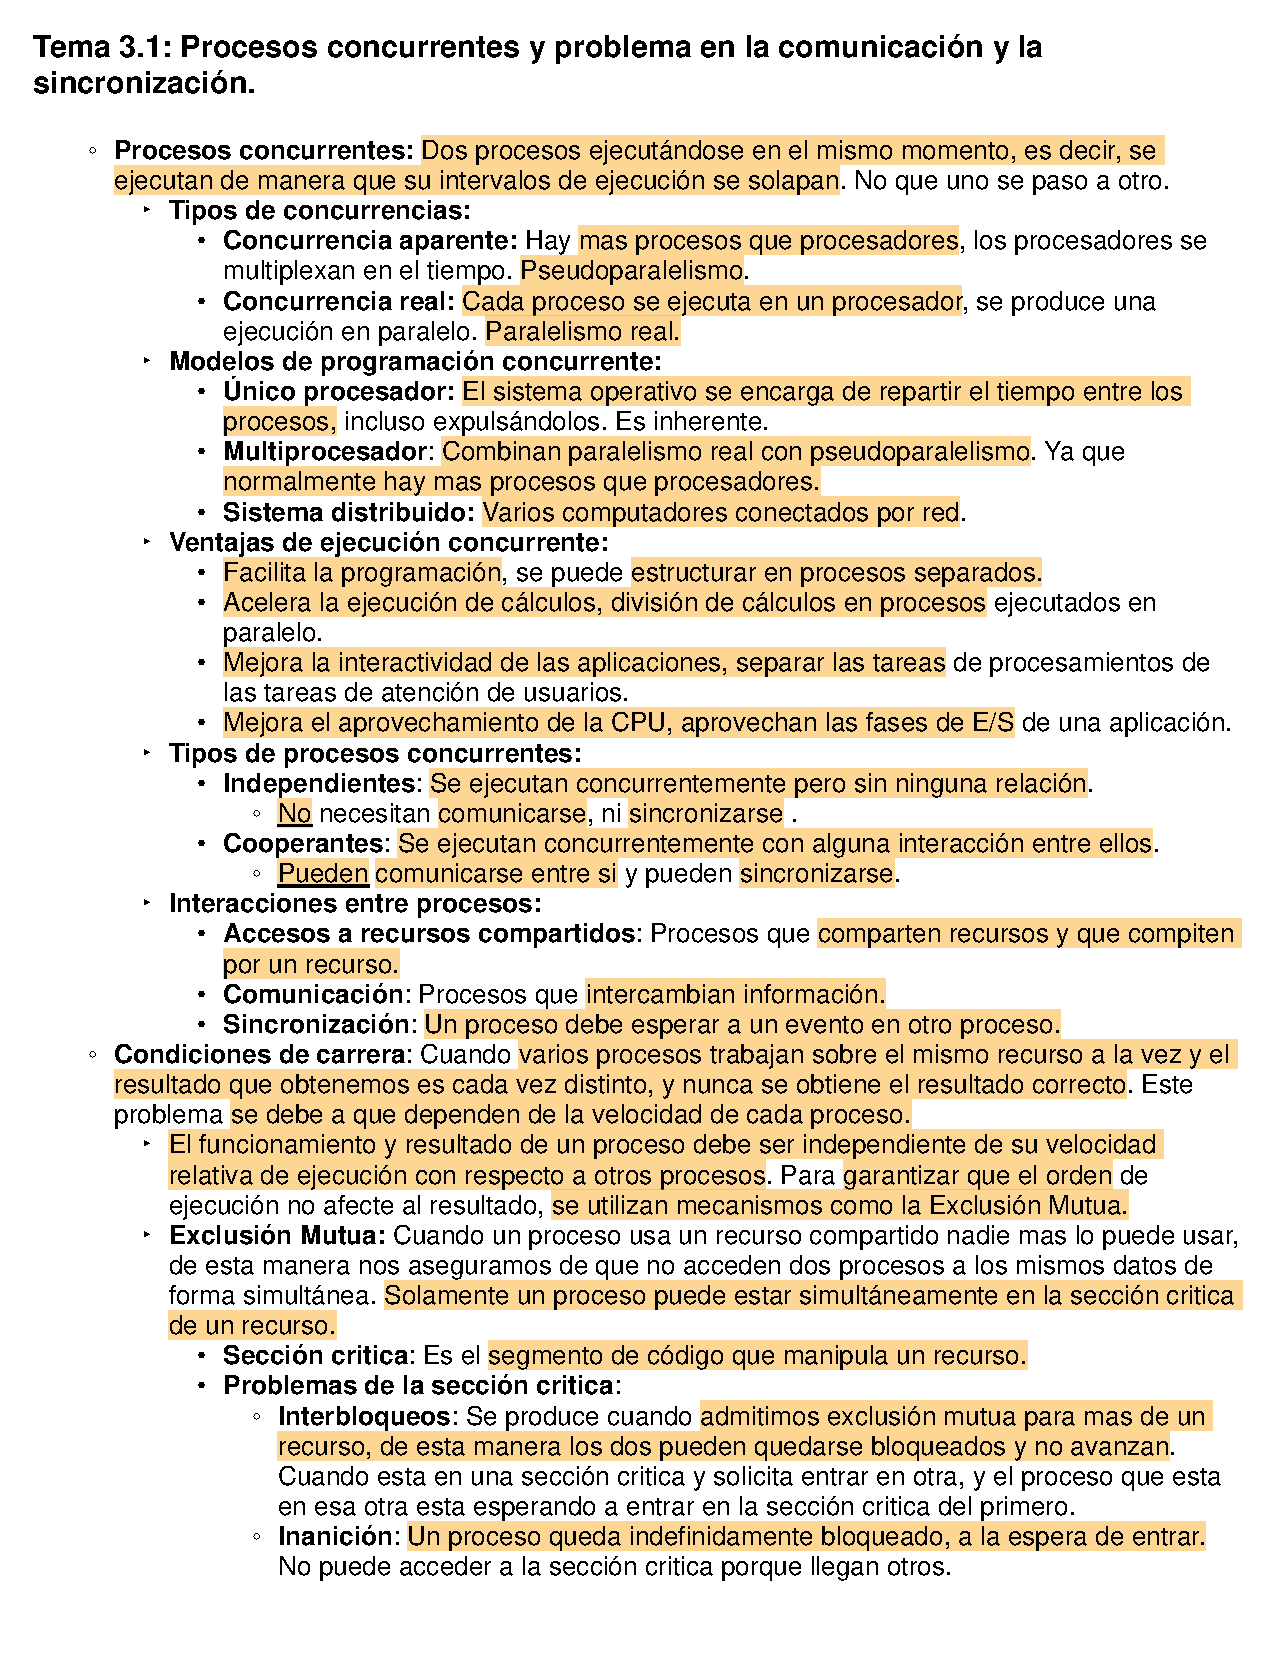
\includepdf[pages=-]{docs/Tema_3_SO.pdf}
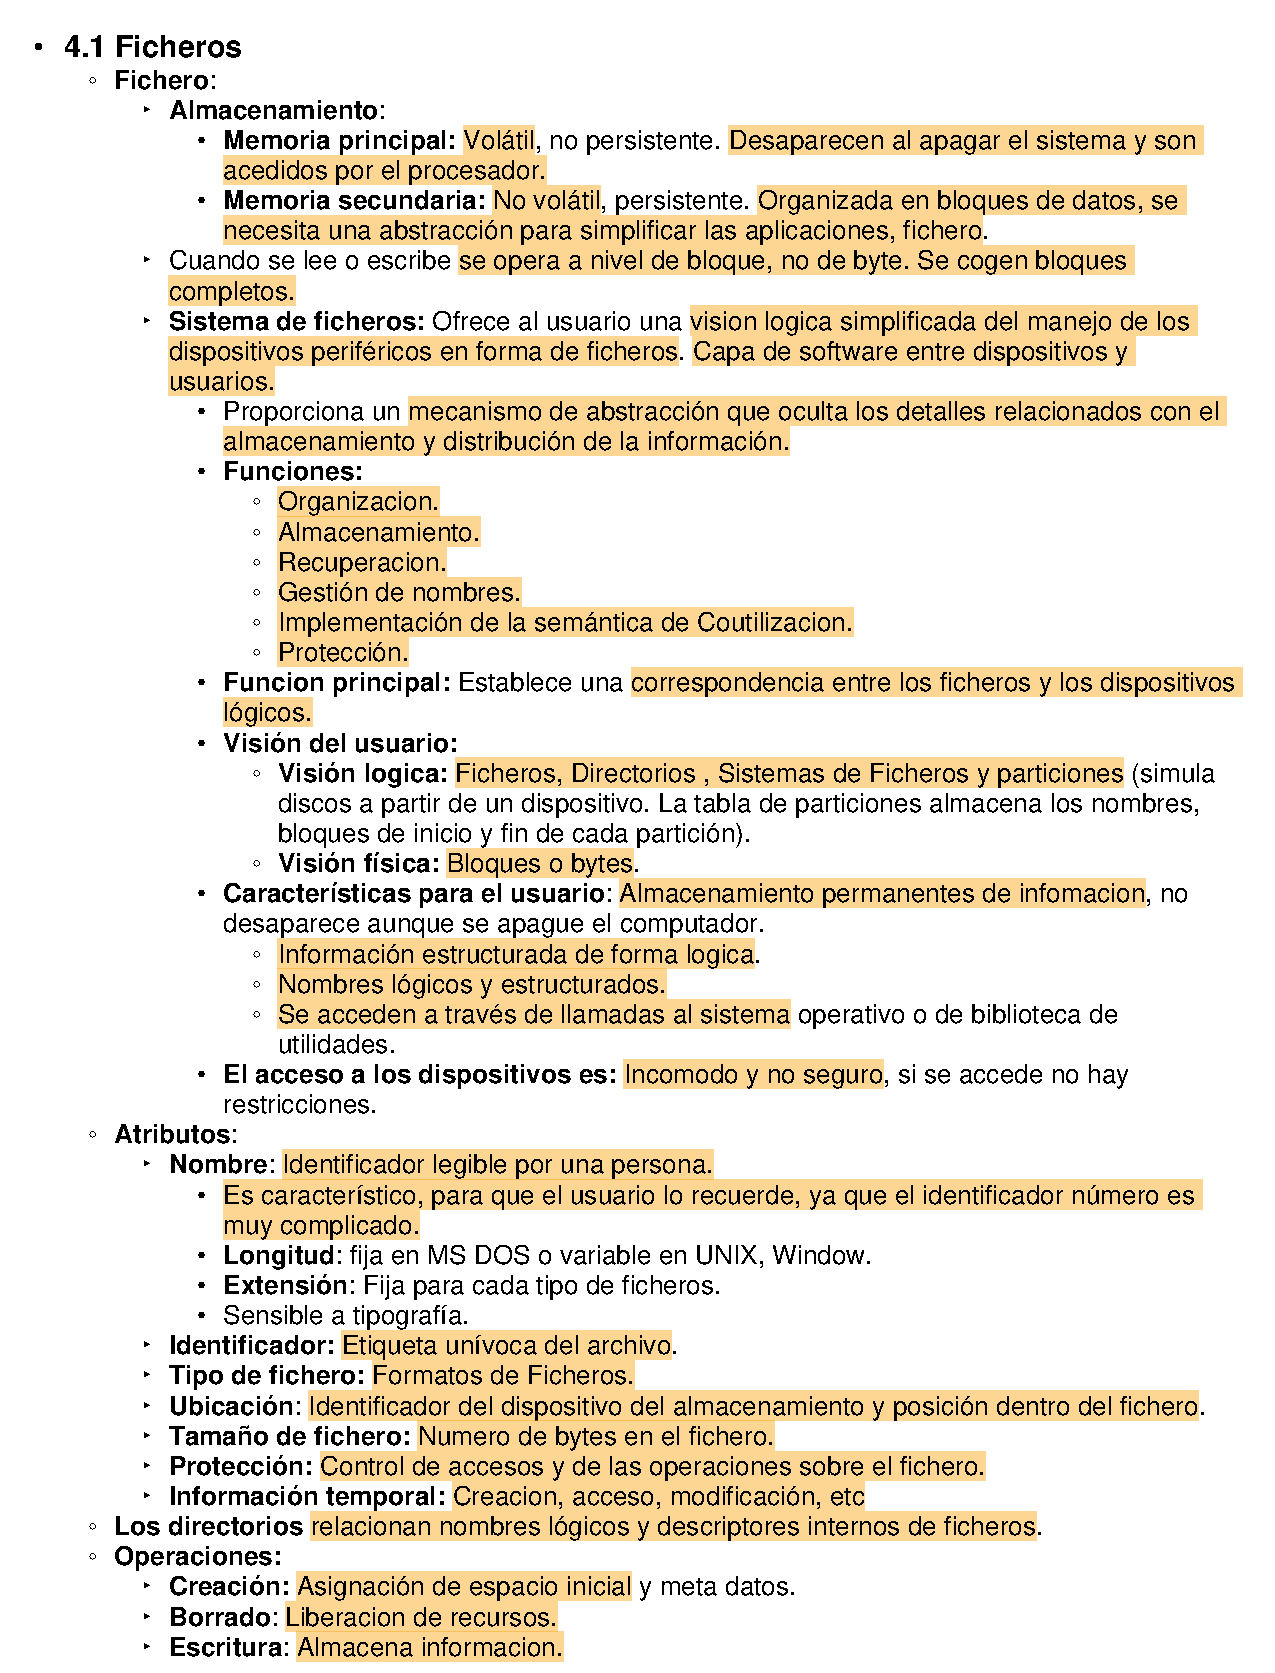
\includepdf[pages=-]{docs/Tema_4_SO.pdf}

\includepdf[pages=-]{docs/Tema_4.2_Directorios.pdf}

\includepdf[pages=-]{docs/Tema_4.3_Sistemas_Ficheros_Servicios_Ficheros.pdf}

\part{Teoría}
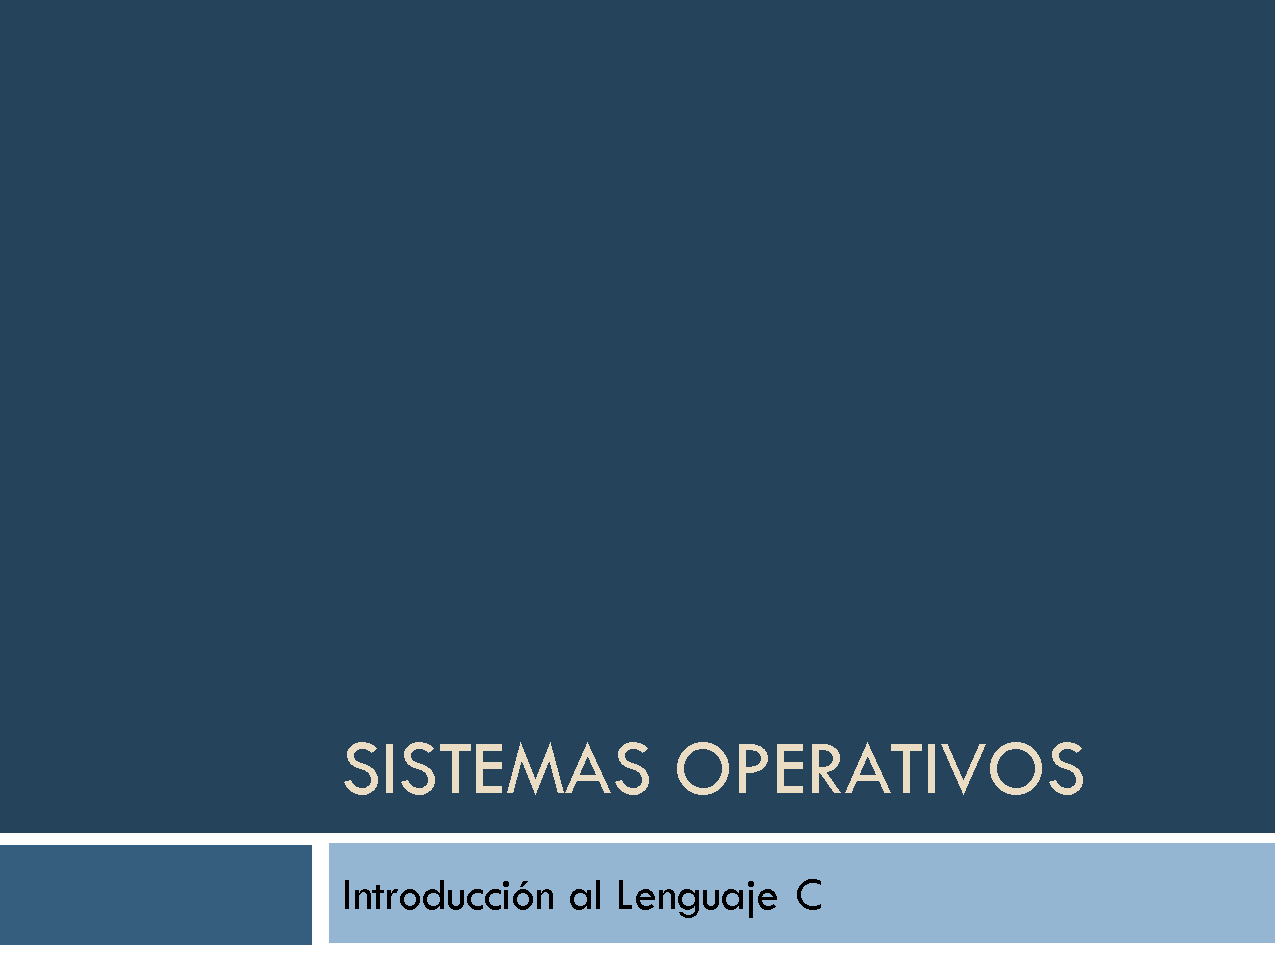
\includepdf[pages=-]{docs/Introduccion_al_Lenguaje_C_(1).pdf}
\includepdf[pages=-]{docs/Presentacion_1.1_Introduccion_y_Conceptos.pdf}
\includepdf[pages=-]{docs/Presentacion_1.2_Servicios_del_SO.pdf}
\includepdf[pages=-]{docs/Presentacion_2.1_Introduccion_a_Gestion_de_Procesos.pdf}
\includepdf[pages=-]{docs/Presentacion_2.2_Planificacion_de_procesos.pdf}
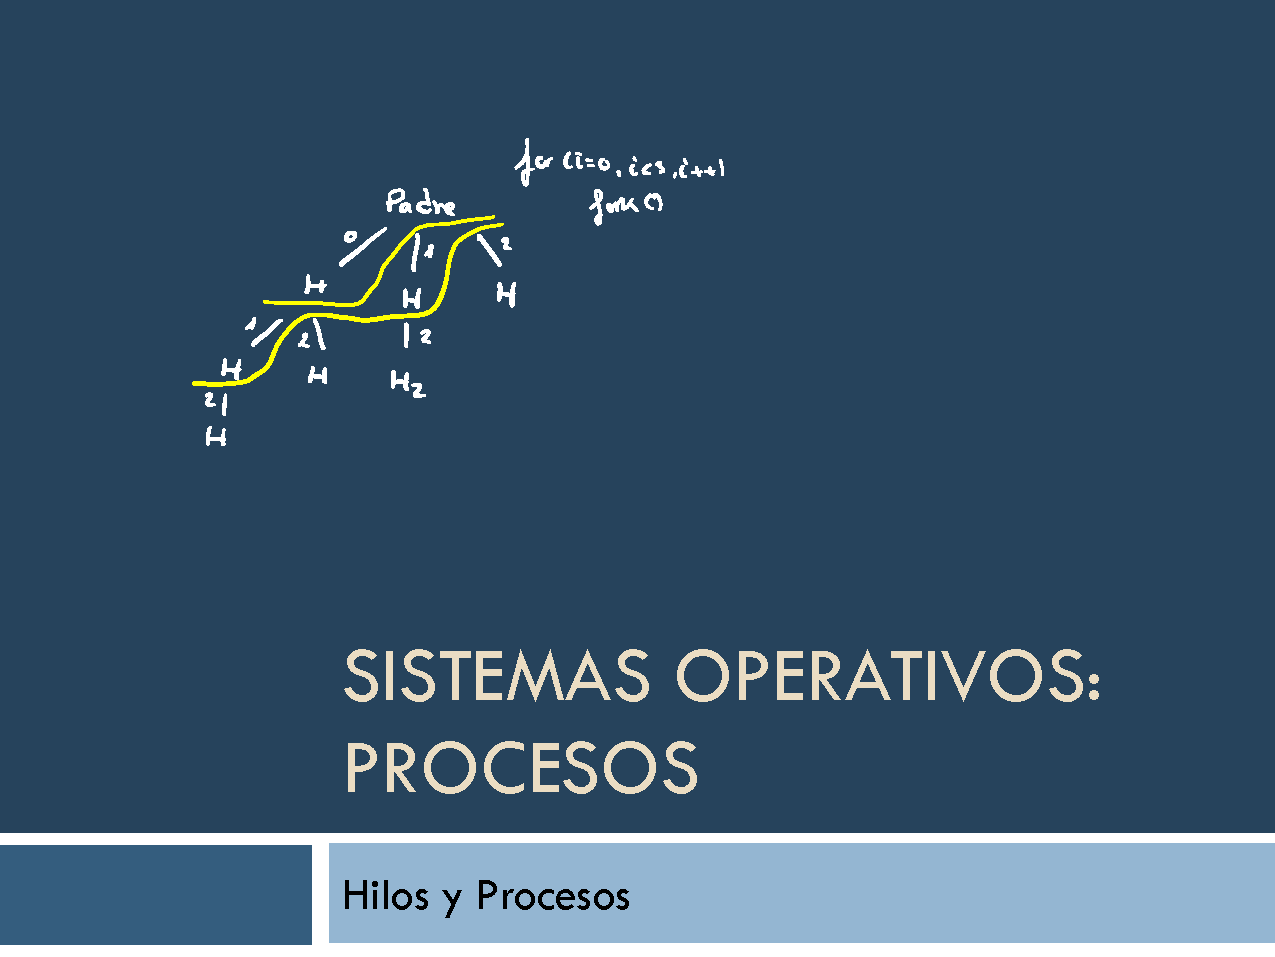
\includepdf[pages=-]{docs/Presentacion_2.3_Hilos_y_Procesos.pdf}
\includepdf[pages=-]{docs/Presentacion_2.4_Senales_excepciones.pdf}
\includepdf[pages=-]{docs/Presentacion_3.1_Introduccion_y_Conceptos.pdf}
\includepdf[pages=-]{docs/Presentacion_3.2_Hilos_y_Mecanismos_Sincronizacion.pdf}
\includepdf[pages=-]{docs/Presentacion_3.3_Desarrollo_Servidores_Concurrentes.pdf}

\includepdf[pages=-]{docs/Presentacion_4.1_Ficheros_.pdf}

\includepdf[pages=-]{docs/Problemas_frecuentes_con_el_lenguaje_C.pdf}
\includepdf[pages=-]{docs/Sesion_2_Problemas_lenguaje_C.pdf}

\includepdf[pages=-]{docs/Sesion_6_Llamadas_al_sistema.pdf}
\includepdf[pages=-]{docs/Sesion_10_Procesos.pdf}
\includepdf[pages=-]{docs/Sesion_12_Tuberias_.pdf}

\includepdf[pages=-]{docs/Sesion_28_Sistema_de_ficheros.pdf}

\part{Ejercicios C}
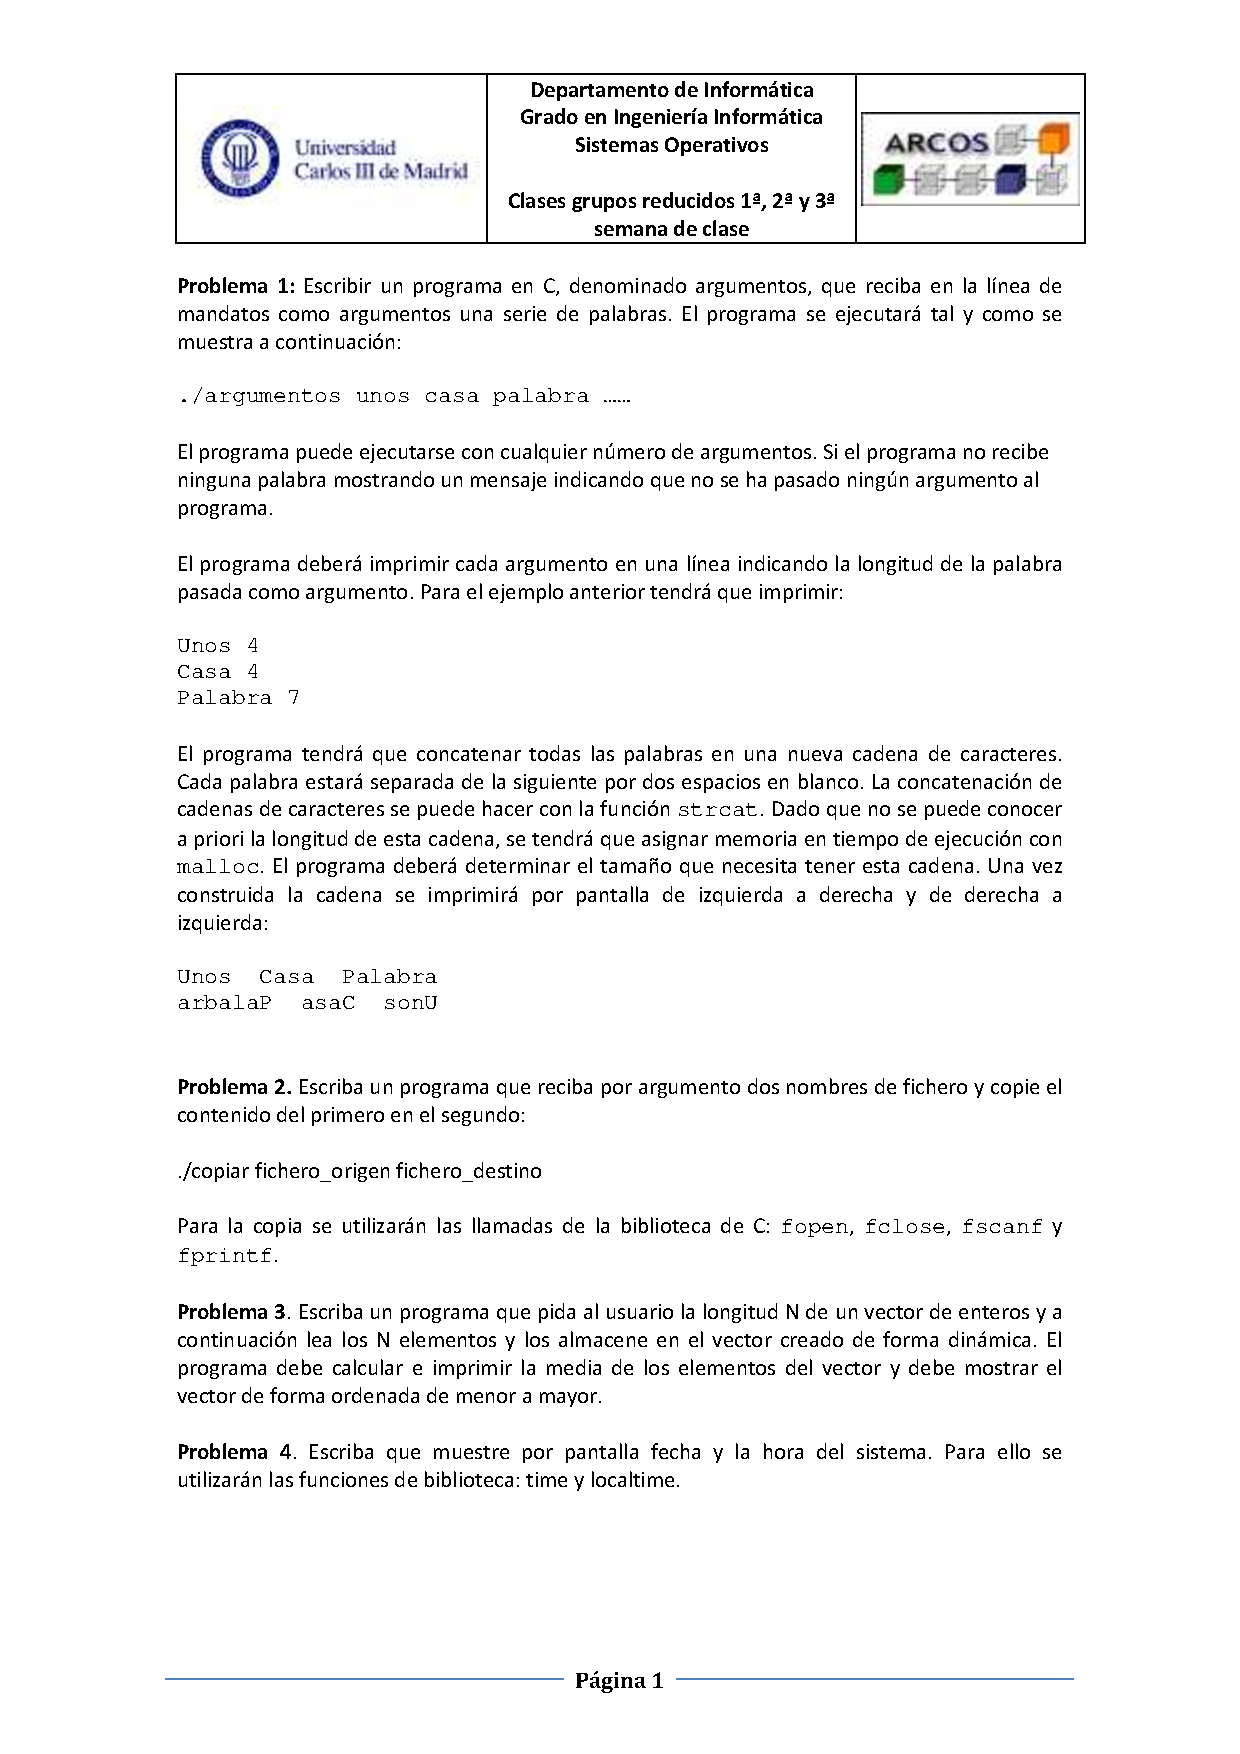
\includepdf[pages=-]{docs/ejercicios-c-2.pdf}
\includepdf[pages=-]{docs/Ejercicios_C.pdf}

\includepdf[pages=-]{docs/03-Problemas_frecuentes_con_el_lenguaje_C.pdf}

\part{Ejercicios teoría y calculo}

\includepdf[pages=-]{docs/01-Problemas_lenguaje_C-01.pdf}
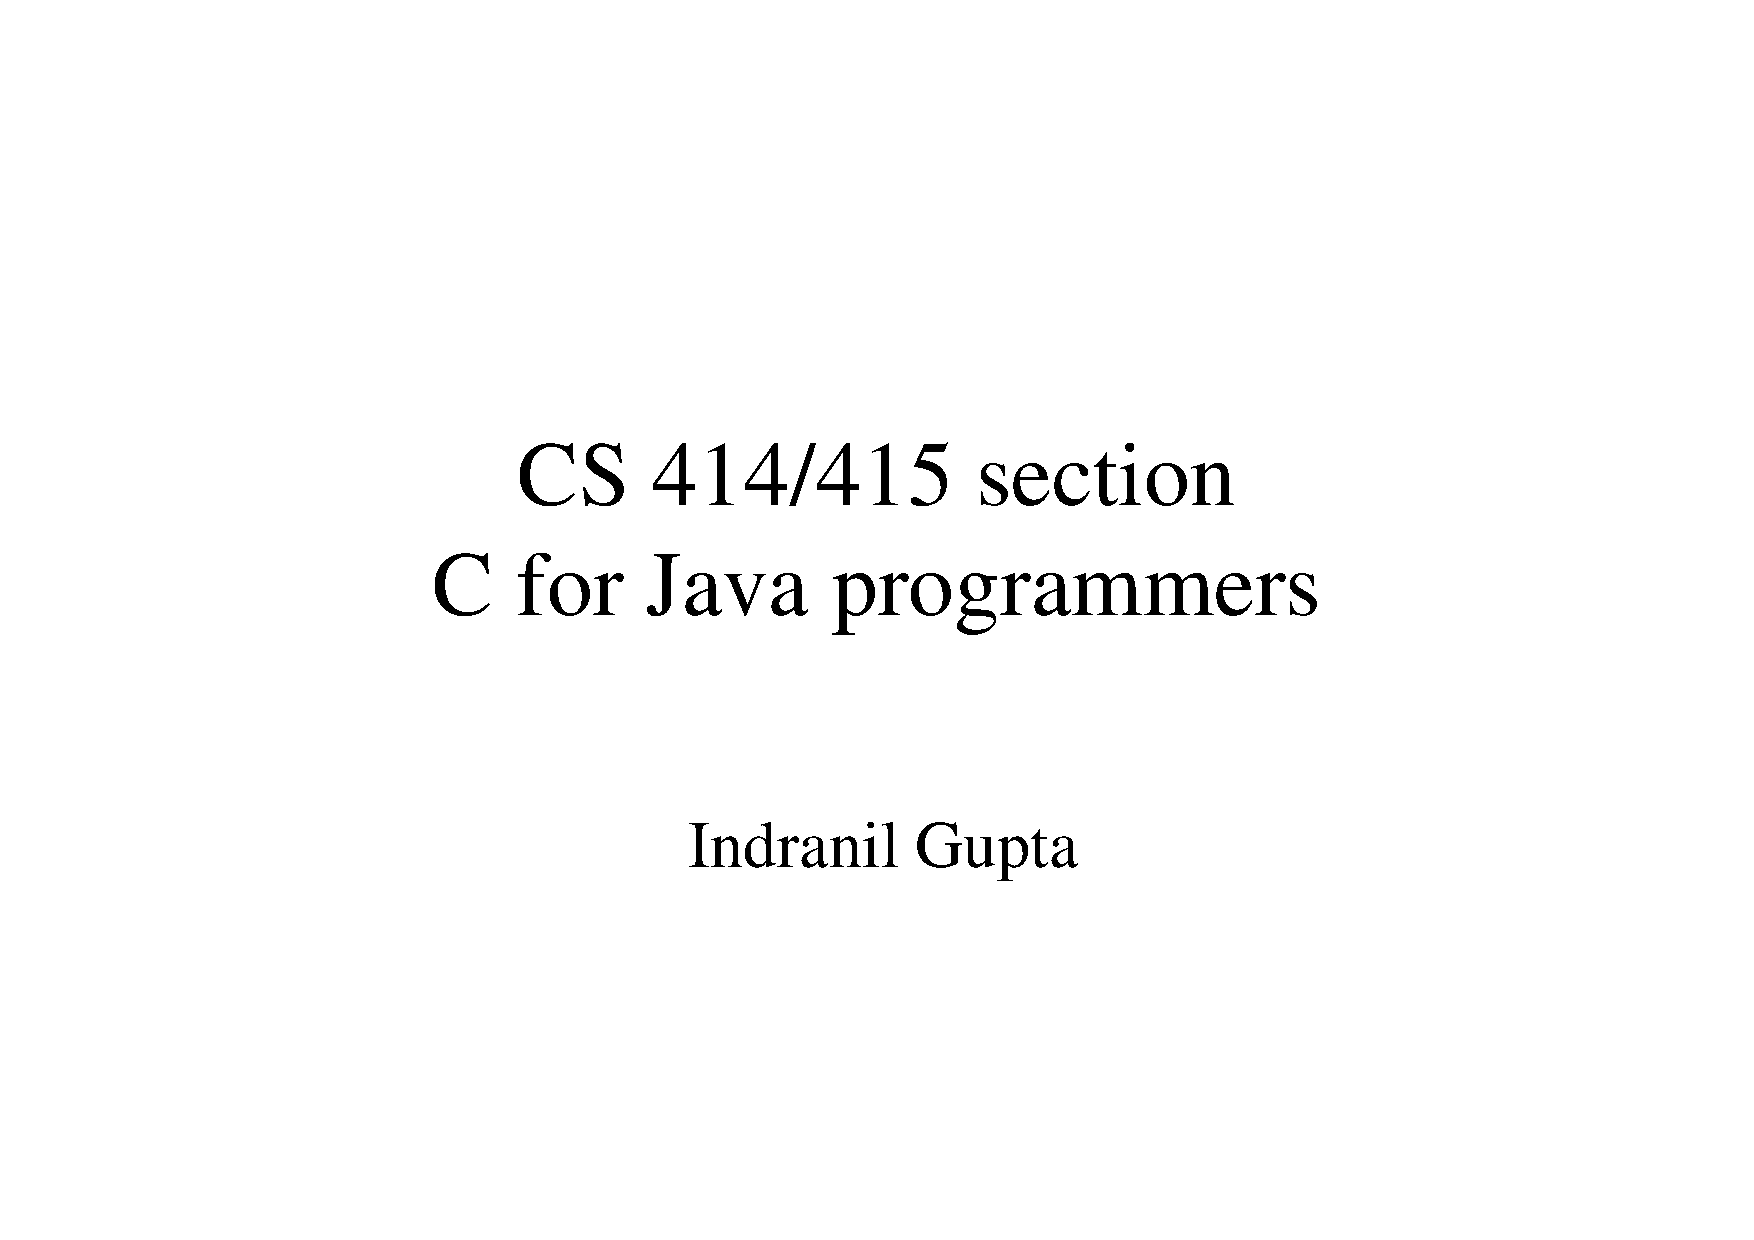
\includepdf[pages=-]{docs/02-c_for_java_programmers.pdf}

\includepdf[pages=-]{docs/04-Llamadas_al_sistema.pdf}
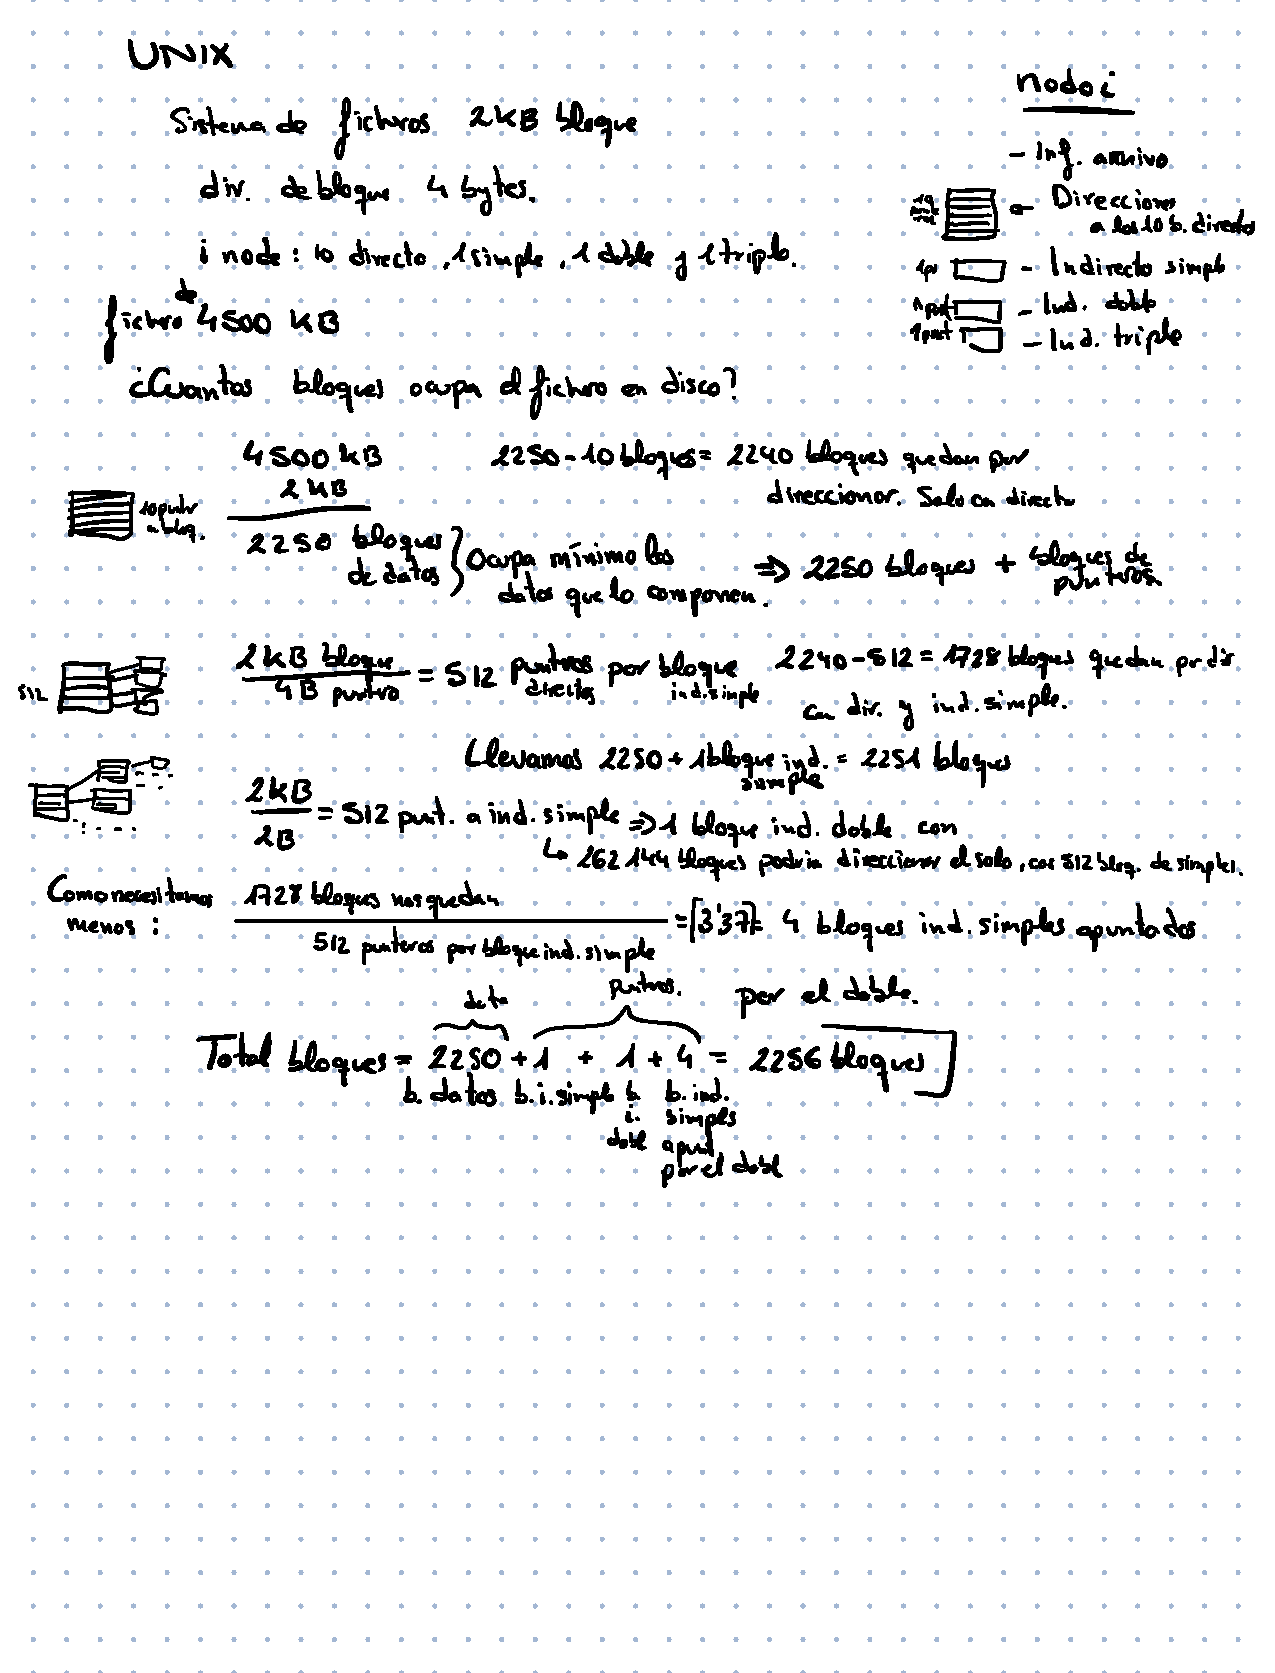
\includepdf[pages=-]{docs/EJ1_T5_L11.pdf}
\includepdf[pages=-]{docs/EJ1_T5_L12.pdf}
\includepdf[pages=-]{docs/EJ1_T5_L13.pdf}
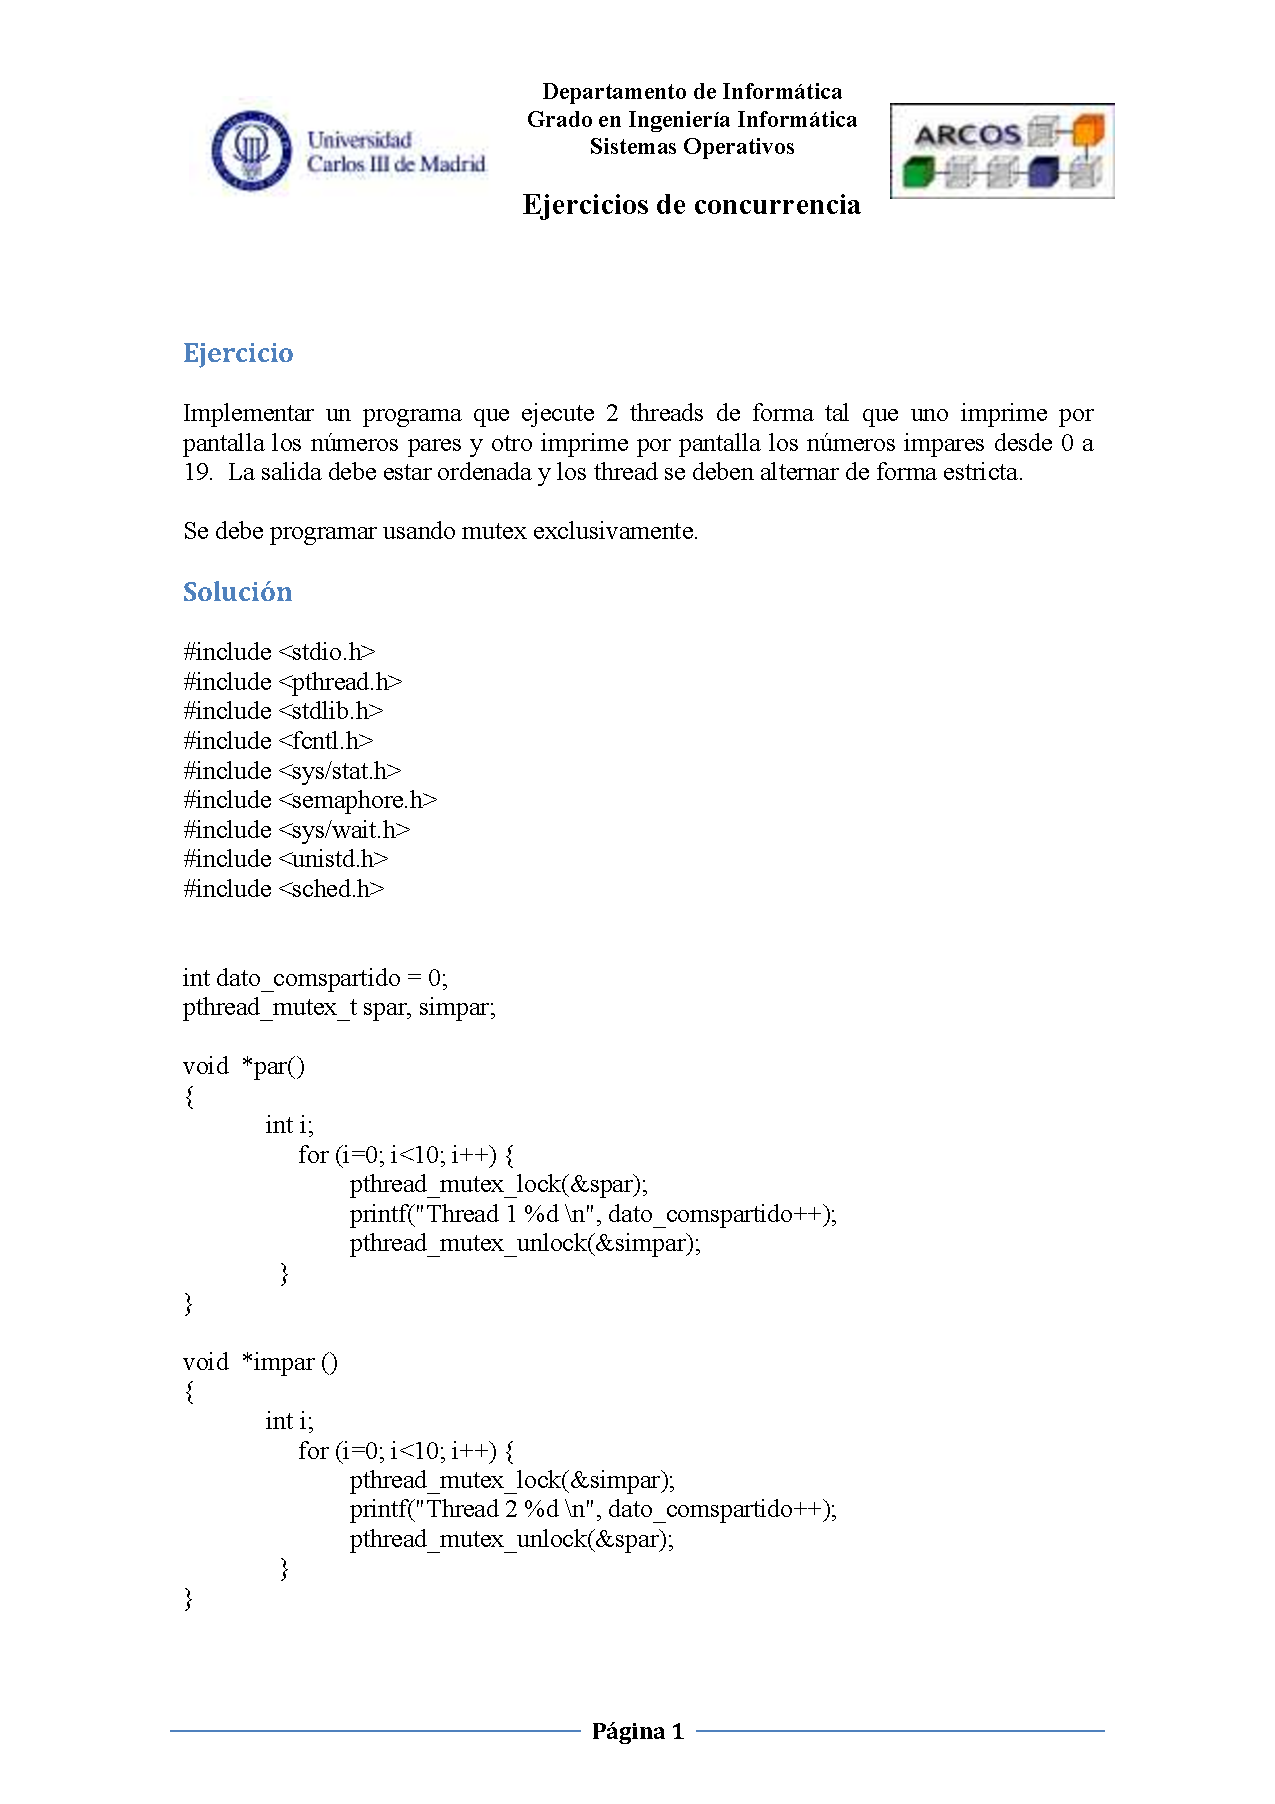
\includepdf[pages=-]{docs/Ejercicios_3-2.pdf}
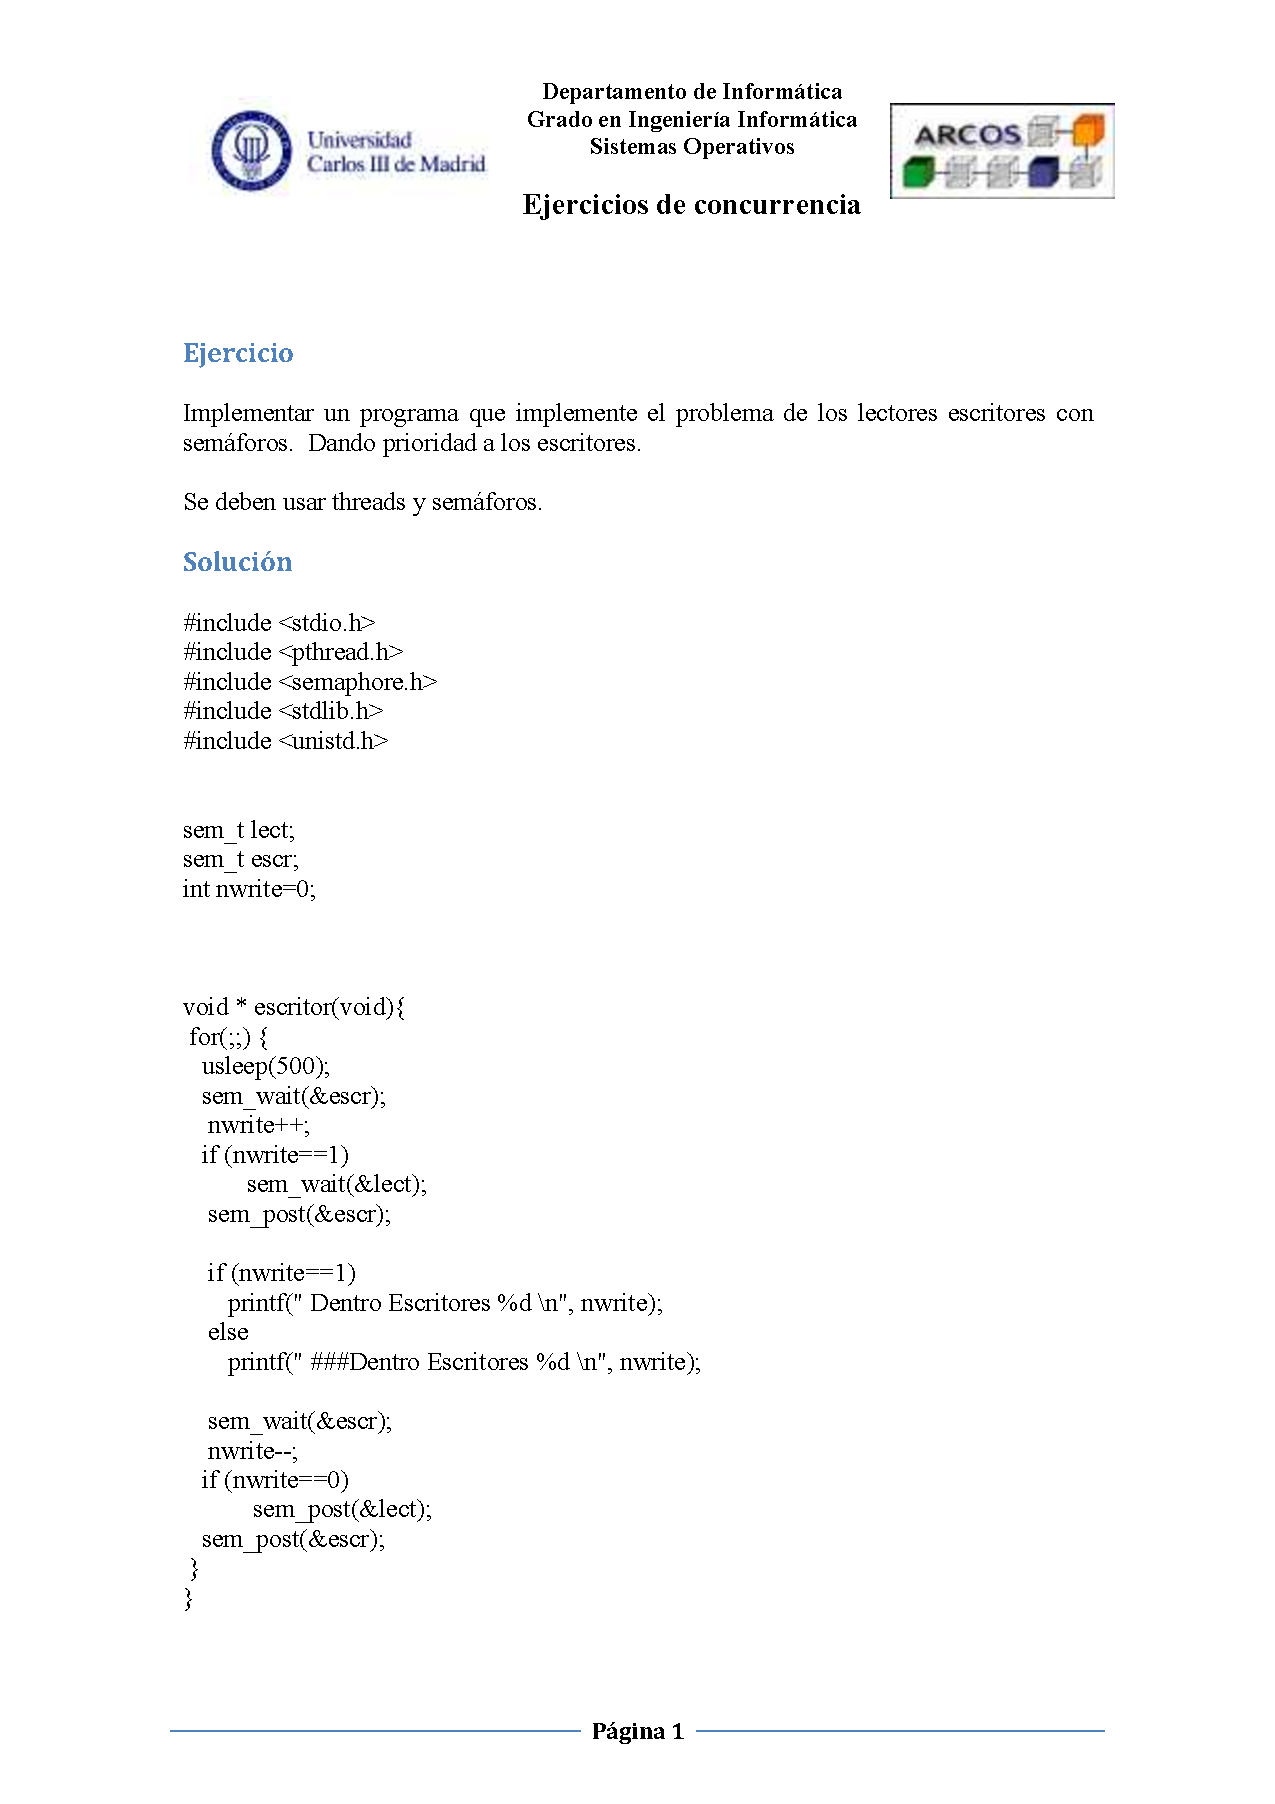
\includepdf[pages=-]{docs/Ejercicios_3-3.pdf}
\includepdf[pages=-]{docs/Ejercicios_3-4_.pdf}
\includepdf[pages=-]{docs/Ejercicios_3-6.pdf}
\includepdf[pages=-]{docs/Ejercicios_C_2.pdf}
\includepdf[pages=-]{docs/Ejercicios_C.pdf}
\includepdf[pages=-]{docs/Ejercicios_Pizarra_SO.pdf}
\includepdf[pages=-]{docs/Ejercicios_T_1.1.pdf}
\includepdf[pages=-]{docs/Ejercicios_T_1.2.pdf}
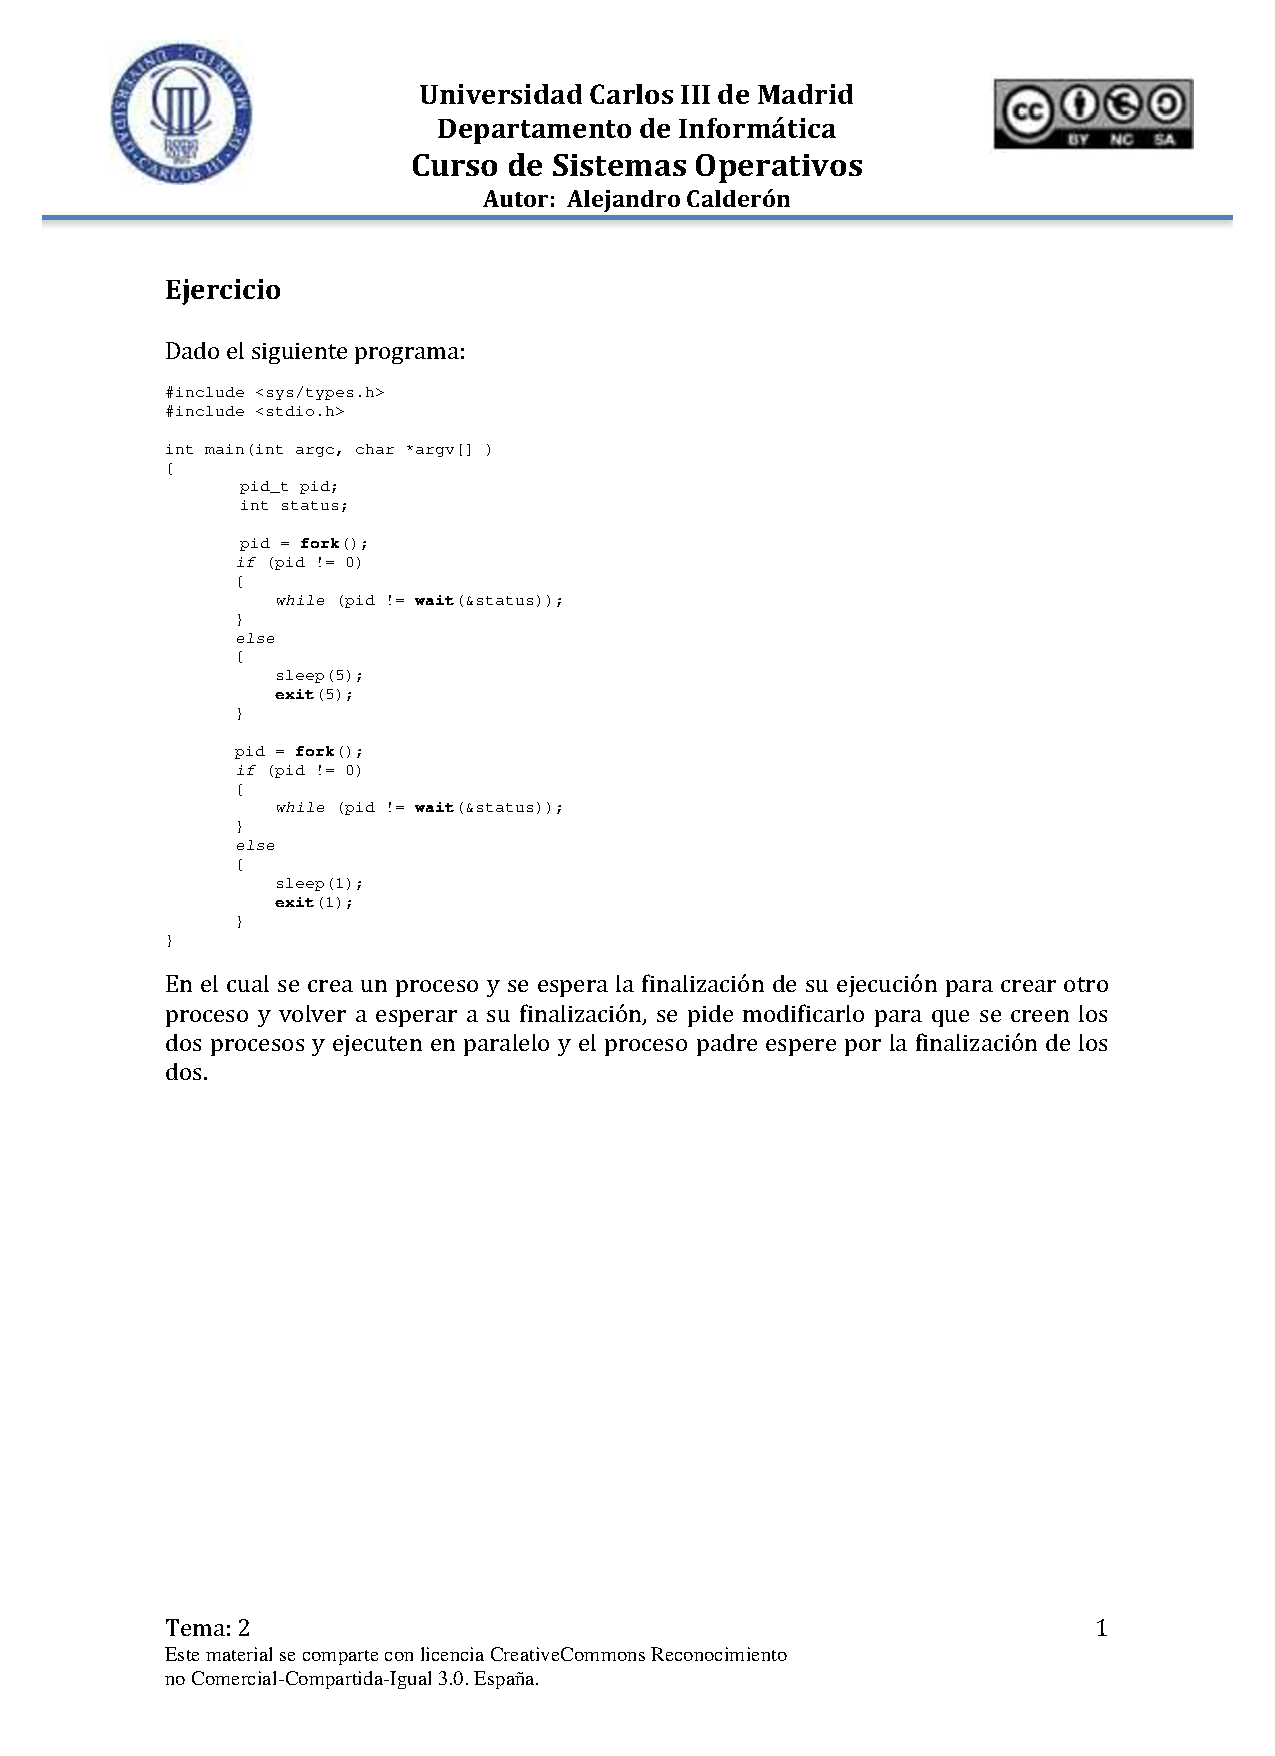
\includepdf[pages=-]{docs/Ejercicios_T_2.1.pdf}
\includepdf[pages=-]{docs/Ejercicios_T_2.2.pdf}
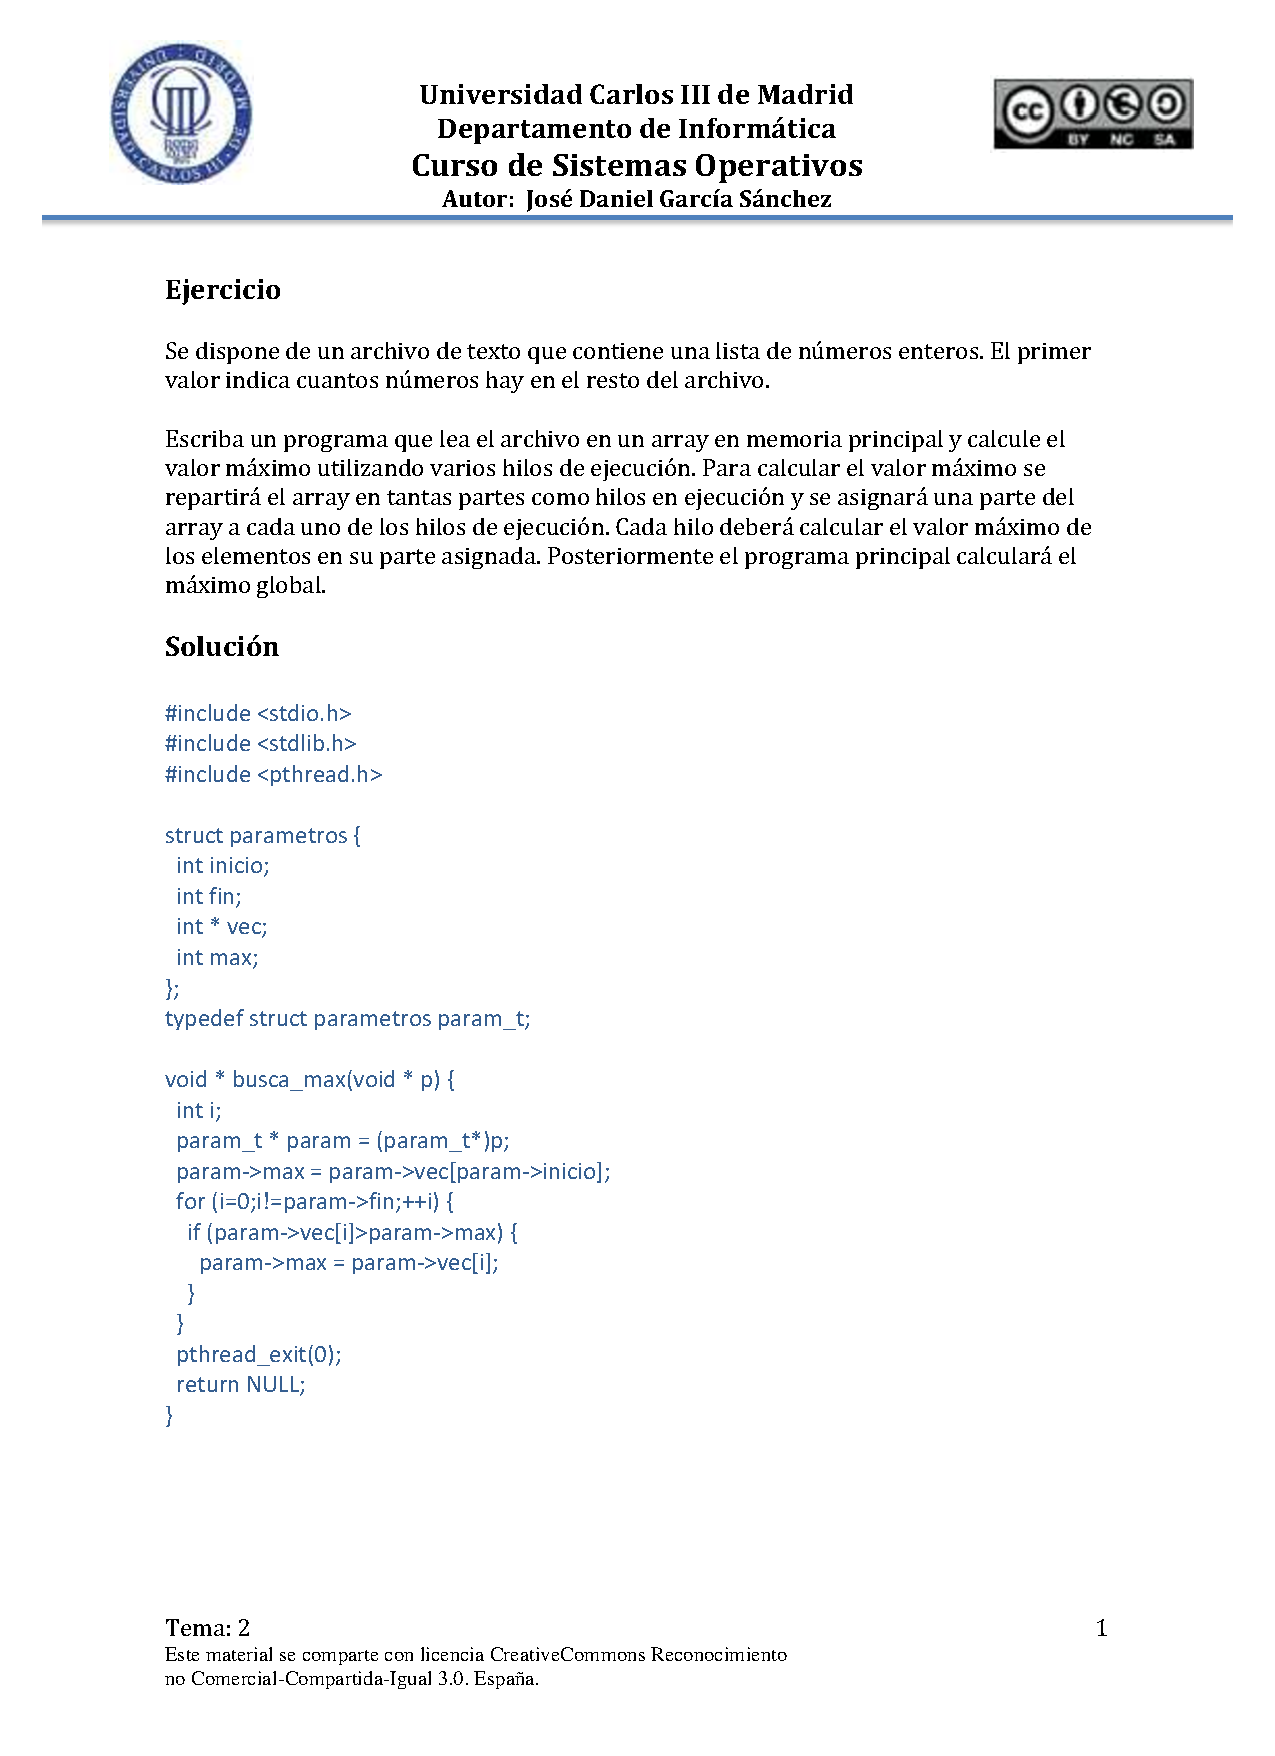
\includepdf[pages=-]{docs/Ejercicios_T_2.3.pdf}
\includepdf[pages=-]{docs/Ejercicios_T_3.0_con_Soluciones_SSOO.pdf}
\includepdf[pages=-]{docs/Ejercicios_T_3.0_SSOO.pdf}
\includepdf[pages=-]{docs/Ejercicios_T_3.1.pdf}
\includepdf[pages=-]{docs/Ejercicios_T_3.2.pdf}
\includepdf[pages=-]{docs/Ejercicios_T_3.3.pdf}
\includepdf[pages=-]{docs/Ejercicios_T_4.1.pdf}
\includepdf[pages=-]{docs/Ejercicios_T_4.2.pdf}
\includepdf[pages=-]{docs/Ejercicios_T_4.3.pdf}
\includepdf[pages=-]{docs/ejercicios-18-03.pdf}
\includepdf[pages=-]{docs/Nota_13_may_2020_9_36_25.pdf}
\includepdf[pages=-]{docs/Nota_20_may_2020_1_47_58.pdf}
\includepdf[pages=-]{docs/Nota_28_abr_2020_12_41_04.pdf}
\includepdf[pages=-]{docs/pipes-sincronizacion.pdf}
\includepdf[pages=-]{docs/Practica_1._Llamadas_al_sistema.pdf}
\includepdf[pages=-]{docs/Practica_2._MiniShell.pdf}
\includepdf[pages=-]{docs/sem-nombre-par-impar.pdf}

\part{Test}
\includepdf[pages=-]{docs/SSOO_AutoTest_1.pdf}
\includepdf[pages=-]{docs/SSOO_Autotest_2.pdf}
\includepdf[pages=-]{docs/SSOO_Autotest_3.pdf}
\includepdf[pages=-]{docs/SSOO_Autotest_soluciones.pdf}

\part{Exámenes}
\includepdf[pages=-]{docs/2009-grado-ssoo-examen-junio-extraordinario-colme-v2.pdf}
\includepdf[pages=-]{docs/2009-ssoo-ordinario-1p.pdf}
\includepdf[pages=-]{docs/2009-ssoo-ordinario-2p-sol.pdf}
\includepdf[pages=-]{docs/2009-ssoo-ordinario-2p.pdf}
\includepdf[pages=-]{docs/2009-ssoo-parcial-sol.pdf}
\includepdf[pages=-]{docs/2009-ssoo-parcial.pdf}
\includepdf[pages=-]{docs/2009grado-ssoo-examen-junio-extraordinario-colme-test.pdf}
\includepdf[pages=-]{docs/2010-ssoo-colme-parcial-sol.pdf}
\includepdf[pages=-]{docs/2010-ssoo-colme-parcial.pdf}
\includepdf[pages=-]{docs/2010-ssoo-ordinario-sol.pdf}
\includepdf[pages=-]{docs/2010-ssoo-parcial-sol-b.pdf}
\includepdf[pages=-]{docs/2010-ssoo-parcial-sol.pdf}
\includepdf[pages=-]{docs/2011-ssoo-extrordinario-sol.pdf}
\includepdf[pages=-]{docs/2013-Parcial-G83-A-Sol.pdf}
\includepdf[pages=-]{docs/2013-Parcial-G83-B-Sol.pdf}
\includepdf[pages=-]{docs/2013-Parcial-Jorge-Sol.pdf}
\includepdf[pages=-]{docs/ejercicios_procesos_senyales_y_planificacion.pdf}
\includepdf[pages=-]{docs/Examen_1_SOL.pdf}
\includepdf[pages=-]{docs/Examen_1P_enero-2010_SOL.pdf}
\includepdf[pages=-]{docs/Examen_1P_enero-2010.pdf}
\includepdf[pages=-]{docs/Examen_2_SOL.pdf}
\includepdf[pages=-]{docs/Examen_2P_enero-2010.pdf}
\includepdf[pages=-]{docs/Examen_3_SOL.pdf}
\includepdf[pages=-]{docs/Examen_extraordinario_junio-2010.pdf}
\includepdf[pages=-]{docs/Examen_extraordinario_ssoo_junio-2010_Solucion_(2).pdf}
\includepdf[pages=-]{docs/Examen_extraordinario_ssoo_junio-2010.pdf}
\includepdf[pages=-]{docs/examen-extraordinario-2014-2015-sol.pdf}
\includepdf[pages=-]{docs/examen-ordinario-2014-2015-solucion.pdf}
\includepdf[pages=-]{docs/examEnero2012ssooParte1-publicar.pdf}
\includepdf[pages=-]{docs/ExamExtraordSSOOjun2010v240610.pdf}
\includepdf[pages=-]{docs/ExSSOOen2013.pdf}
\includepdf[pages=-]{docs/ExSSOOjun2010_SOL.pdf}
\includepdf[pages=-]{docs/ExSSOOJun2011-definitivo.pdf}
\includepdf[pages=-]{docs/ExSSOOJun2011v3-sol.pdf}
\includepdf[pages=-]{docs/ExSSOOsep2010_SOLv030910_(2).pdf}
\includepdf[pages=-]{docs/ExSSOOsep2010_SOLv030910.pdf}
\includepdf[pages=-]{docs/grado-ssoo-examen-junio-extraordinario-colme-v2.pdf}
\includepdf[pages=-]{docs/II-SSOO-2006-junio-colmenarejo-parcial01-G81.pdf}
\includepdf[pages=-]{docs/II-SSOO-2007-junio-1pE-sol.pdf}
\includepdf[pages=-]{docs/II-SSOO-2007-junio-2pE-sol.pdf}
\includepdf[pages=-]{docs/II-SSOO-2007-sept-sol.pdf}
\includepdf[pages=-]{docs/itig-ssoo-2008-junio-sol.pdf}
\includepdf[pages=-]{docs/itig-ssoo-2008-sept-sol.pdf}
\includepdf[pages=-]{docs/parcial_(2).pdf}
\includepdf[pages=-]{docs/parcial_SSOO_sol_colme50-1.pdf}
\includepdf[pages=-]{docs/parcial-solucion_(2).pdf}
\includepdf[pages=-]{docs/parcial-solucion.pdf}
\includepdf[pages=-]{docs/parcial.pdf}
\includepdf[pages=-]{docs/Primer_Parcial_SSOO_2010-2011-grs-81-82-83.pdf}
\includepdf[pages=-]{docs/Primer_Parcial_SSOO_2010-2011-grs-84-85-solucion.pdf}
\includepdf[pages=-]{docs/Primer_Parcial_SSOO_2010-2011-grs-84-85.pdf}
\includepdf[pages=-]{docs/primer-parcial-8182-octubre-2009.pdf}
\includepdf[pages=-]{docs/primer-parcial-8384-octubre-2009.pdf}
\includepdf[pages=-]{docs/primer-parcial-colme-2008-2009.pdf}
\includepdf[pages=-]{docs/solexjun2006.pdf}
\includepdf[pages=-]{docs/solexjun2007.pdf}
\includepdf[pages=-]{docs/solexsep2007.pdf}
\includepdf[pages=-]{docs/solexsept2006.pdf}
\includepdf[pages=-]{docs/SSOO_extraordinario_2014_Mod1-sol.pdf}
\includepdf[pages=-]{docs/SSOO_extraordinario_jun_2013_problemas-solucion.pdf}
\includepdf[pages=-]{docs/SSOO_extraordinario_jun_2013_v1_-_sol.pdf}
\includepdf[pages=-]{docs/SSOO_g_ii_primer_parcial_8485_octubre-2010_solucion.pdf}
\includepdf[pages=-]{docs/SSOO_g_ii_primer_parcial_Colmenarejo_octubre-2010_solucion.pdf}
\includepdf[pages=-]{docs/SSOO_ordinaria_2014_solucion.pdf}
\includepdf[pages=-]{docs/SSOO_ordinario_jun_2013_v1-sol.pdf}
\includepdf[pages=-]{docs/SSOO_parcial_2014_g8182_solucion.pdf}
\includepdf[pages=-]{docs/SSOO_parcial_2014_Mod6_sol.pdf}
\includepdf[pages=-]{docs/SSOO_parcial_2015_g8182TipoASolucionv120315b.pdf}
\includepdf[pages=-]{docs/SSOO_primer_parcial_81_2013.pdf}
\includepdf[pages=-]{docs/ssoo-final-test-modelo-C_sol.pdf}
\includepdf[pages=-]{docs/ssoo-ordinario-febreo-2011.pdf}
\includepdf[pages=-]{docs/ssoo-ssh-actividad-2013.pdf}

\part{Practica 1. Llamadas al sistema}
\includepdf[pages=-]{docs/ssoo_p1_100405951_100405834.pdf}
\includepdf[pages=-]{docs/notas_p1_ssoo_81.pdf}
\includepdf[pages=-]{docs/p1_llamadas_al_sistema_19-20.pdf}

\part{Practica 2. MiniShell}
\includepdf[pages=-]{docs/p2_minishell_enunciado_19-20.pdf}
\includepdf[pages=-]{docs/p2_minishell_transparencias_19-20.pdf}
\includepdf[pages=-]{docs/tuberias.pdf}
\includepdf[pages=-]{docs/ssoo_p2_100405951_100405834.pdf}

\part{Practica 3. Multi-hilo}
\includepdf[pages=-]{docs/ssoo_p3_multithread_19-20.pdf}
\includepdf[pages=-]{docs/ssoo_p3_100405951_100405834.pdf}

\part{Recursos}
\includepdf[pages=-]{docs/errores-frecuentes-C.pdf}
\includepdf[pages=-]{docs/Guia_C.pdf}
\includepdf[pages=-]{docs/Lenguaje-C.pdf}
\includepdf[pages=-]{docs/Principales_comandos_del_editor_vi.pdf}

\end{document}